
\documentclass[12pt,a4paper]{article}

%-------------------- Package Imports --------------------%
\usepackage[utf8]{inputenc}
\usepackage[T1]{fontenc}
\usepackage{lmodern}               % Improved font rendering
\usepackage{geometry}              % Page geometry
\geometry{margin=1in}             % Set margins to your preference
\usepackage[hidelinks]{hyperref}              % Clickable links and refs
\usepackage{graphicx}              % For images
\usepackage{enumitem}              % Better control of list environments
\usepackage{xcolor}                % Color text if needed
\usepackage{makeidx}               % For creating an index
\makeindex                         % Initialize index creation
\usepackage[style=alphabetic]{biblatex} % BibLaTeX for references
\addbibresource{references.bib}    % External .bib file for references
% \usepackage[toc,acronym]{glossaries}   % Glossaries and acronyms
% \usepackage[automake]{glossaries-extra}
% \makeglossaries  
% \newacronym{gcd}{GCD}{Greatest Common Divisor}
% \makenoidxglossaries


\usepackage[style=long,nonumberlist,toc,xindy,acronym,nomain]{glossaries}
\makeglossaries  

\usepackage[utf8]{inputenc}

\usepackage{mdframed} % For framed boxes
\usepackage{tikz}
\usetikzlibrary{arrows.meta, positioning}







% A bunch of glossary entries
    \newglossaryentry{monero-wallet (v0.1.0)}{
        name={\protect\texttt{monero-wallet (v0.1.0)}},
        description={A standard library crate, with the corresponding entry point at  \path{/wallet/src/lib.rs}. Handles all wallet functionality}
    }

    \newglossaryentry{monero-simple-request-rpc (v0.1.0)}{
        name={\protect\texttt{monero-simple-request-rpc (v0.1.0)}},
        description={A standard library crate, with the corresponding entry point at  \path{/rpc/simple-request/src/lib.rs}. Default RPC to avoid external dependences, e.g. reqwest}
    }

    \newglossaryentry{monero-rpc (v0.1.0)}{
        name={\protect\texttt{monero-rpc (v0.1.0)}},
        description={A standard library crate, with the corresponding entry point at \path{/rpc/src/lib.rs}. It defines traits and types for retrieving blockchain data, managing transactions, and selecting decoy outputs for ring signatures. The crate implements both standard JSON-RPC and Monero-specific binary protocols, with a focus on security when dealing with potentially untrusted nodes.}
    }

    \newglossaryentry{monero-serai (v0.1.4-alpha)}{
        name={\protect\texttt{monero-serai (v0.1.4-alpha)}},
        description={A standard library crate, with the corresponding entry point at \path{/src/lib.rs}. This is the overall transaction library}
    }

    \newglossaryentry{monero-address (v0.1.0)}{
        name={\protect\texttt{monero-address (v0.1.0)}},
        description={A standard library crate, with the corresponding entry point at \path{/wallet/address/src/lib.rs}. Handles Monero addresses}
    }

    \newglossaryentry{monero-borromean (v0.1.0)}{
        name={\protect\texttt{monero-borromean (v0.1.0)}},
        description={A standard library crate, with the corresponding entry point at \path{/ringct/borromean/src/lib.rs}. Employs no modules, and untested. Handles Borromean signatures and Borromean range proofs}
    }


    \newglossaryentry{monero-bulletproofs (v0.1.0)}{
        name={\protect\texttt{monero-bulletproofs (v0.1.0)}},
        description={A standard library crate, with the corresponding entry point at \path{/ringct/bulletproofs/src/lib.rs}. Handles original bulletproofs and bulletproofs plus}
    }

    \newglossaryentry{monero-clsag (v0.1.0)}{
        name={\protect\texttt{monero-clsag (v0.1.0)}},
        description={A standard library crate, with the corresponding entry point at \path{/ringct/clsag/src/lib.rs}. Handles CLSAG ring signatures and a FROST-like thresholdization.}
    }

    \newglossaryentry{monero-mlsag (v0.1.0)}{%
      name={\protect\texttt{monero-mlsag (v0.1.0)}},
      description={A Rust crate located at \path{/networks/monero/ringct/mlsag/src/lib.rs} providing
      Multilayered Linkable Spontaneous Anonymous Group (MLSAG) ring signatures for the Monero protocol.
      Maintains core MLSAG structures (\texttt{RingMatrix} and \texttt{Mlsag}) and an aggregate
      matrix builder. Implements zeroization, but needs expanded testing and finer-grained error handling.}
    }

    \newglossaryentry{monero-primitives (v0.1.0)}{
        name={\protect\texttt{monero-primitives (v0.1.0)}},
        description={A standard library crate, with the corresponding entry point at \path{/primitives/src/lib.rs}.}
    }

    \newglossaryentry{monero-generators (v0.4.0)}{
        name={\protect\texttt{monero-generators (v0.4.0)}},
        description={A standard library crate, with the corresponding entry point at \path{/generators/src/lib.rs}. Handles hashing to elliptic curve group elements and computing fixed generators for use in the Monero protocol}
    }

    \newglossaryentry{monero-io (v0.1.0)}{
        name={\protect\texttt{monero-io (v0.1.0)}},
        description={A standard library crate with entry point at \path{/io/src/lib.rs}. Employs no modules, and untested.  Handles reading and writing various data structures used in Monero protocol computations (e.g.\ bytes, scalars, group elements, lists whose entries are the same type)}
    }
    
    \newglossaryentry{decoys-module}{
        name={\protect\path{/wallet/src/decoys.rs}},
        description={The module handling decoys.}
    }

    \newglossaryentry{extra-module}{
        name={\protect\path{/wallet/src/extra.rs}},
        description={The module handling the extra field of transactions.}
    }

    \newglossaryentry{output-module}{
        name={\protect\path{/wallet/src/output.rs}},
        description={The module handling transaction outputs.}
    }

    \newglossaryentry{scan-module}{
        name={\protect\path{/wallet/src/scan.rs}},
        description={The module handling scanning.}
    }

    \newglossaryentry{view-pair-module}{
        name={\protect\path{/wallet/src/view_pair.rs}},
        description={The module handling the (public-spend, private-view) keys.}
    }

    \newglossaryentry{send-module}{
        name={\protect\path{/wallet/src/send/mod.rs}},
        description={The module handling the sending transactions.}
    }

    \newglossaryentry{block-module}{
        name={\protect\texttt{block}},
        description={A module in \texttt{monero-serai} handling Monero block structures and related functionality}
    }

    \newglossaryentry{merkle-module}{
        name={\protect\path{/src/merkle.rs}},
        description={Module for handling Merkle trees}
    }

    \newglossaryentry{ring-signatures-module}{
        name={\protect\texttt{ring\_signatures}},
        description={A module in \texttt{monero-serai} implementing Monero's ring signature scheme for transaction privacy}
    }

    \newglossaryentry{ringct-module}{
        name={\protect\texttt{ringct}},
        description={A module in \texttt{monero-serai} implementing RingCT (Ring Confidential Transaction) functionality, including bulletproofs and CLSAG signatures}
    }

    \newglossaryentry{transaction-module}{
        name={\protect\texttt{transaction}},
        description={A module in \texttt{monero-serai} containing data structures and functionality for Monero transactions, including different transaction versions and serialization/deserialization}
    }

    \newglossaryentry{base58-module}{
        name={\protect\path{/wallet/address/src/base58check.rs}},
        description={Module for handling base58 enc/dec}
    }

    \newglossaryentry{monero-serai-entry-point}{
        name={\protect\path{/src/lib.rs}},
        description={Entry point for the monero-serai transaction library}.
    }
    
    \newglossaryentry{wallet-tests}{
        name={\protect\path{/wallet/src/tests/runner/mod.rs}},
        description={Testing module for \texttt{monero wallet (v0.1.0)}}
    }

    \newglossaryentry{wallet-entry-point}{
        name={\protect\path{/wallet/src/lib.rs}},
        description={The entry point to the \gls{monero-wallet (v0.1.0)} crate}
    }

    \newglossaryentry{monero-simple-request-rpc-entry-point}{
        name={\protect\path{/rpc/simple-request/src/lib.rs}},
        description={The entry point to the \gls{monero-simple-request-rpc (v0.1.0)} crate}
    }
    
    \newglossaryentry{monero-rpc-entry-point}{
        name={\protect\path{/rpc/src/lib.rs}},
        description={Module for handling RPC calls for communicating on the Monero network.}.
    }


    \newglossaryentry{monero-serai-tests}{
        name={\protect\path{/src/tests/mod.rs}},
        description={Testing module for handling \gls{monero-serai (v0.1.4-alpha)} tests}
    }

    \newglossaryentry{address-tests}{
        name={\protect\path{/wallet/address/src/tests.rs}},
        description={Testing module for \gls{monero-address (v0.1.0)} tests}
    }

    
    \newglossaryentry{borromean-entry-point}{
        name={\protect\path{/ringct/borromean/src/lib.rs}},
        description={Entry point to \gls{monero-borromean (v0.1.0)}}
    }

    
    \newglossaryentry{bulletproofs-entry-point}{
        name={\protect\path{/ringct/bulletproofs/src/lib.rs}},
        description={Entry point to \gls{monero-bulletproofs (v0.1.0)}}
    }

    
    \newglossaryentry{bp-batch-verifier-module}{
        name={\protect\path{/ringct/bulletproofs/src/batch_verifier.rs}},
        description={Module for handling batch verification of bulletproofs}
    }

    \newglossaryentry{bp-core-module}{
        name={\protect\path{/ringct/bulletproofs/src/core.rs}},
        description={Module for handling the core folding computation of bulletproofs.}
    }


    \newglossaryentry{bp-point-vector-module}{
        name={\protect\path{/ringct/bulletproofs/src/point_vector.rs}},
        description={Module for handling the vectors of group elements in bulletproofs.}
    }


    \newglossaryentry{bp-scalar-vector-module}{
        name={\protect\path{/ringct/bulletproofs/src/scalar_vector.rs}},
        description={Module for handling the vectors of field elements/scalars in bulletproofs.}
    }


    \newglossaryentry{bp-original-module}{
        name={\protect\path{/ringct/bulletproofs/src/original/mod.rs}},
        description={Module for handling the original bulletproofs}
    }

    \newglossaryentry{bp-plus-module}{
        name={\protect\path{/ringct/bulletproofs/src/plus/mod.rs}},
        description={Module for handling bulletproofs plus}
    }

    \newglossaryentry{bp-test-module}{
        name={\protect\path{/ringct/bulletproofs/src/plus/mod.rs}},
        description={Module for handling bulletproofs tests}
    }

    \newglossaryentry{monero-clsag-entry-point}{
        name={\protect\path{/ringct/clsag/src/lib.rs}},
        description={Entry point for \gls{monero-clsag (v0.1.0)}}
    }
   
    \newglossaryentry{clsag-multisig-module}{
        name={\protect\path{/ringct/clsag/src/multisig.rs}},
        description={Module for handling CLSAG signatures.}
    } 

    \newglossaryentry{clsag-tests}{
        name={\protect\path{/ringct/clsag/src/tests.rs}},
        description={Test module for CLSAG signatures.}
    } 

    \newglossaryentry{monero-mlsag-entry-point}{
        name={\protect\path{/ringct/mlsag/src/lib.rs}},
        description={Entry point for \gls{monero-mlsag (v0.1.0)}}
    } 

    \newglossaryentry{monero-primitives-entry-point}{
        name={\protect\path{/primitives/src/lib.rs}},
        description={Entry point for \gls{monero-primitives (v0.1.0)}}
    } 


    \newglossaryentry{unreduced-scalar-module}{
        name={\protect\path{/primitives/src/unreduced_scalar.rs}},
        description={Module for handling unreduced scalars.}
    } 


    \newglossaryentry{monero-primitives-tests}{
        name={\protect\path{/primitives/src/tests.rs}},
        description={Testing module for \gls{monero-primitives (v0.1.0)}}
    } 

    \newglossaryentry{monero-generators-entry-point}{
        name={\protect\path{/generators/src/lib.rs}},
        description={Entry point for \gls{monero-generators (v0.4.0)}}
    } 

    \newglossaryentry{hash-to-point-module}{
        name={\protect\path{/generators/src/hash_to_point.rs}},
        description={Module for handling hashing data to elliptic curve group elements}
    } 
    
    \newglossaryentry{monero-generators-tests}{
        name={\protect\path{/generators/src/tests/mod.rs}},
        description={Testing module for \gls{monero-generators (v0.4.0)}}
    } 

    \newglossaryentry{monero-io-entry-point}{
        name={\protect\path{/io/src/lib.rs}},
        description={Entry point for \gls{monero-io (v0.1.0)}}
    } 
    
    \newglossaryentry{monero-address-entry-point}{
        name={\protect\path{/wallet/address/src/lib.rs}},
        description={Entry point for \gls{monero-address (v0.1.0)}}
    } 

    
    
    \newglossaryentry{eventuality-module}{
        name={\protect\path{/wallet/src/send/eventuality.rs}},
        description={Module for handling \gls{eventualities}}
    } 
    
    
    \newglossaryentry{send-multisig-module}{
        name={\protect\path{/wallet/src/send/multisig.rs}},
        description={Module for handling multisig transactions}
    } 

    
    \newglossaryentry{send-tx-module}{
        name={\protect\path{/wallet/src/send/tx.rs}},
        description={Module for handling sending transactions}
    } 
    
    \newglossaryentry{send-tx-keys-module}{
        name={\protect\path{/wallet/src/send/tx_key.rs}},
        description={Module for handling keys in sending transactions}
    } 

    \newglossaryentry{eventualities}{
        name={Eventualities},
        description={A struct for handling the eventual output from \gls{SignableTransaction}s.}
    } 




    

%-------------------- Title, Author, Date --------------------%
\title{\textbf{Audit of \path{serai/networks/monero/}}}
% \author{Brandon Goodell \\ \texttt{brandon@cypherstack.com}}
\author{
    Joshua Babb\thanks{Cypher Stack} \\ % First line for the first author
    \and
    Brandon Goodell\footnotemark[1] \\ % First line for the second author
    \and
    Rigo Salazar\footnotemark[1] \\ % First line for the third author
    % \and
    % Freeman Slaughter\footnotemark[1] \\
    % \and 
    % Luke Szramowski\footnotemark[1] \\
    % \and 
    % kayaba
}
\date{\today}

%===================== DOCUMENT START =====================%
\begin{document}

\maketitle

\tableofcontents
\clearpage

%-------------------- Section: Introduction / Scope --------------------%
\section{Introduction}

We review the Rust implementation of FROSTLASS, the \path{/serai-dex/serai/networks/monero/} directory in commit \texttt{48db06f} by \texttt{KayabaNerve} of the GitHub repository at \url{github.com/serai-dex/serai}. This directory contains a Rust implementation of Monero wallet functionality, together with a new approach to using FROST for threshold signing. All files, folders, and subfolders of \path{/serai-dex/serai/networks/monero/} are in scope for the audit, except not the subfolder \path{/serai-dex/serai/networks/monero/verify-chain/}.


\section{General Findings}

Overall, the code is consistent, neat, clean, and efficient. The following practices are used throughout.
\begin{itemize}
\item Use of \texttt{LazyLock} for thread-safe lazy initialization.  % https://github.com/serai-dex/serai/blob/48db06f901952b24bb38d7c7e256f798f08512cd/networks/monero/generators/src/lib.rs#L6 and https://github.com/serai-dex/serai/blob/48db06f901952b24bb38d7c7e256f798f08512cd/networks/monero/generators/src/lib.rs#L29 and https://github.com/serai-dex/serai/blob/48db06f901952b24bb38d7c7e256f798f08512cd/networks/monero/generators/src/lib.rs#L35
\item Constant-time group operations from \texttt{curve25519-dalek}.  % https://github.com/serai-dex/serai/blob/48db06f901952b24bb38d7c7e256f798f08512cd/networks/monero/generators/src/lib.rs#L10
\item Constant-time hash-to-point mapping.  % https://github.com/serai-dex/serai/blob/48db06f901952b24bb38d7c7e256f798f08512cd/networks/monero/generators/src/hash_to_point.rs#L1
\item Implement \texttt{Zeroize} and \texttt{ZeroizeOnDrop} for sensitive data.  % eg. https://github.com/serai-dex/serai/blob/48db06f901952b24bb38d7c7e256f798f08512cd/networks/monero/primitives/src/lib.rs#L82
\item Perform careful bounds checking when handling anonymity sets/tuples. % https://github.com/serai-dex/serai/blob/48db06f901952b24bb38d7c7e256f798f08512cd/networks/monero/primitives/src/lib.rs#L165-L167

\item Use utility types for vectors of \texttt{Scalar} and \\\texttt{EdwardsPoint} for safe indexing and algebraic operations. 

\item Seal code with \texttt{sealed} modules, enforcing that certain traits are private to certain modules, so that only types defined within the same module can implement it.

\item Use \texttt{Arc<Mutex>} for safe concurrent access during authentication of state and for nonce management.

\item Manage thread-safe connections through \texttt{Arc<Mutex<(Option<(WwwAuthenticateHeader, u64)>, Client)>>} in the \texttt{monero-rpc} crate.

\item Non-constant time primitives which explicitly match Monero's default wallet implementation.

\item Enforce canonical forms by requiring fully reduced values modulo the group order, canonical forms for point coordinates, and validation of prime-order subgroup membership.

\item Thoroughly tested, including tests against Monero default wallet implementation.
\end{itemize}

Although the codebase is largely robust, the following issues have been identified:
\begin{itemize}
    \item Use of unchecked conversions and the frequent use of \texttt{unwrap()} can lead to runtime panics.
    \item Critical operations (e.g. varint decoding, point decompression, and scalar conversions) lack sufficient error differentiation.
    \item Documentation of complex arithmetic and cryptographic design decisions is sparse, making it harder to verify that every individual line meets security best practices.
    \item Higher-level concerns include the choice of hash functions, inadequate domain separation in transcript construction, and potential vulnerabilities in asynchronous and resource-management patterns.
\end{itemize}

\subsection{Code and Protocol Flow}

\section{Repository Structure}



The repository at \url{github.com/serai-dex/serai} is organized into several top-level directories, including \path{/serai-dex/serai/networks/}, which in turn contains \path{/serai-dex/serai/networks/monero/}.  Figure \ref{fig:directory_structure} describes the target directory structure, where asterisks indicate crates (named in parentheses); the only folder not in scope of this audit is \texttt{verify-chain}. 



\begin{figure}[h]
\centering
\begin{minipage}{0.9\linewidth}
\begin{mdframed}
\begin{verbatim}
/serai-dex/serai/
|-- out_of_scope_files
|-- networks/
    |-- out_of_scope_files
    |-- monero*/ (monero-serai)
        |-- generators*/ (monero-generators)
        |-- io*/ (monero-io)
        |-- primitives*/ (monero-primitives)
        |-- ringct/
            |-- borromean*/ (monero-borromean)
            |-- bulletproofs*/ (monero-bulletproofs)
            |-- clsag*/ (monero-clsag)
            |-- mlsag*/ (monero-mlsag)
        |-- rpc*/ (monero-rpc)
            |-- simple-request*/ (monero-simple-request-rpc)
        |-- src/
        |-- tests/
        |-- verify-chain*/
        |-- wallet*/ (monero-wallet)
            |-- address*/ (monero-address)
\end{verbatim}
\end{mdframed}
\end{minipage}
\caption{Directory structure of the target repository. Everything within \protect\path{/serai-dex/serai/networks/monero} is in scope, except the subfolder \protect\path{/serai-dex/serai/networks/monero/verify-chain/}. Asterisks indicate crates. Crate names are included in parantheses.}
\label{fig:directory_structure}
\end{figure}




% \subsection{Crate Dependencies}

In the following, we omit \texttt{/serai-dex/serai/networks/monero/} from directory references for clarity, with the understanding that all directory references use this as a prefix.

The crates are evocatively named by the data they handle, and mutually depend on each other. Crate dependency is not isomorphic to the file structure. 
Figure \ref{fig:transitive_reduced_dependency_graph} displays these dependencies in the transitive reduction of the directed graph of crate dependencies. Readers should be aware that the transitive reduction of a directed graph $G$ is constructed by removing as many edges as possible without changing the \textit{reachability relation} on pairs of vertices. Thus, not all edges corresponding to direct crate dependency are displayed in Figure \ref{fig:transitive_reduced_dependency_graph}. For example, \texttt{monero-serai} depends directly on \texttt{monero-generators}, \texttt{monero-io}, and \texttt{monero-primitives}.
In Section \ref{sec:crate_summaries}, we present a look at each crate. 

\begin{figure}[h]
\centering
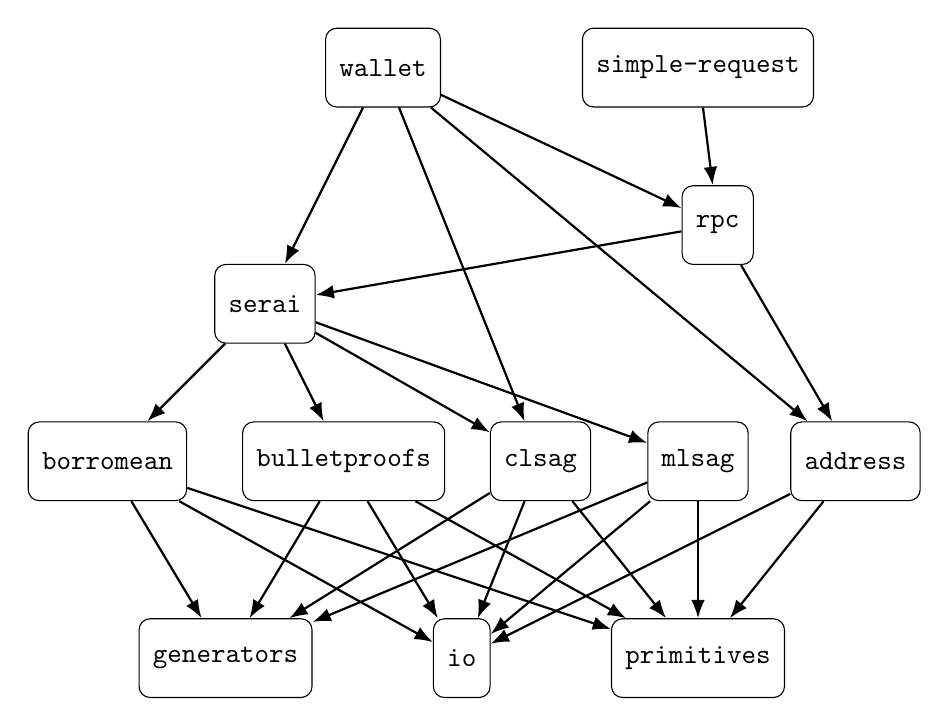
\begin{tikzpicture}[
    scale=1, % Ensure proper scaling
    every node/.style={draw, rectangle, rounded corners, minimum height=1cm, font=\ttfamily, inner sep=5pt, align=center}, % Rectangular nodes
    edge/.style={-{Latex}, thick}
]

% Manually normalized coordinates for a 10x7 aspect ratio
\node (wallet) at (4, 8.5) {wallet};
\node (simple-request) at (8, 8.5) {simple-request};
\node (rpc) at (8.25, 6.5) {rpc};
\node (serai) at (2.5, 5.5) {serai};
\node (address) at (10, 3.5) {address};
\node (mlsag) at (8, 3.5) {mlsag};
\node (clsag) at (6, 3.5) {clsag};
\node (bulletproofs) at (3.5, 3.5) {bulletproofs};
\node (borromean) at (0.5, 3.5) {borromean};
\node (io) at (5, 1) {io};
\node (generators) at (2, 1) {generators};
\node (primitives) at (8, 1) {primitives};

% Edges
\draw[edge] (wallet) -- (rpc);
\draw[edge] (wallet) -- (address);
\draw[edge] (wallet) -- (clsag);
\draw[edge] (wallet) -- (serai);
\draw[edge] (simple-request) -- (rpc);
\draw[edge] (rpc) -- (serai);
\draw[edge] (rpc) -- (address);
\draw[edge] (serai) -- (borromean);
\draw[edge] (serai) -- (bulletproofs);
\draw[edge] (serai) -- (clsag);
\draw[edge] (serai) -- (mlsag);
\draw[edge] (address) -- (io);
\draw[edge] (address) -- (primitives);
\draw[edge] (borromean) -- (io);
\draw[edge] (borromean) -- (generators);
\draw[edge] (borromean) -- (primitives);
\draw[edge] (bulletproofs) -- (io);
\draw[edge] (bulletproofs) -- (generators);
\draw[edge] (bulletproofs) -- (primitives);
\draw[edge] (clsag) -- (io);
\draw[edge] (clsag) -- (generators);
\draw[edge] (clsag) -- (primitives);
\draw[edge] (mlsag) -- (io);
\draw[edge] (mlsag) -- (generators);
\draw[edge] (mlsag) -- (primitives);

\end{tikzpicture}
\caption{The transitive reduction of the graph of crates and their dependencies. Not all edges corresponding to a direct dependency are displayed in a transitive reduction. For example, \texttt{monero-serai} depends directly on \texttt{monero-generators}, \texttt{monero-io}, and \texttt{monero-primitives}, but these edges are not explicitly displayed.}
\label{fig:transitive_reduced_dependency_graph}
\end{figure}

\section{Functionality}

\subsection{Crate Details}\label{sec:crate_summaries}

In this section, we describe each crate name, version, purpose, internal dependencies, and a brief description of crate structure. We use a breadth-first, top-down approach following Figure \ref{fig:transitive_reduced_dependency_graph}. Elements of public APIs (i.e.\ with the modifier \texttt{pub}) have names which are decorated \texttt{thusly}\textsuperscript{\textdagger}, and elements exposed at the crate level (i.e.\ with the modifier \texttt{pub(crate)}) have names which are decorated \texttt{thusly}\textsuperscript{$\Delta$}. We provide links throughout the document to corresponding glossary entries.

% The big itemize starts here

\begin{itemize} 

 \item \gls{monero-wallet (v0.1.0)}
 \begin{itemize}
 \item Purpose: Handle all wallet functionality.
 \item Internal Dependencies: 
 \begin{itemize}
 \item \gls{monero-address (v0.1.0)}\textsuperscript{\textdagger}
 \item \gls{monero-clsag (v0.1.0)}\textsuperscript{\textdagger}
 \item \gls{monero-rpc (v0.1.0)}\textsuperscript{\textdagger}, 
 \item \gls{monero-serai (v0.1.4-alpha)}\textsuperscript{\textdagger}
 \end{itemize}
 \item Structure: A standard library crate, with the corresponding entry point at  \gls{wallet-entry-point}. 
 
 \item Tests at \gls{wallet-tests}.
 \item The \gls{monero-wallet (v0.1.0)} crate employs the following modules.
\begin{itemize}
\item \gls{decoys-module} handles decoy selection with a publicly exposed struct \texttt{OutputWithDecoys}.
\item \gls{extra-module}\textsuperscript{\textdagger} handles the \texttt{extra} field of a transaction.
\item \gls{output-module}\textsuperscript{$\Delta$} handles transaction outputs.
\item \gls{scan-module} handles transaction scanning.
\item \gls{send-module}\textsuperscript{\textdagger} handles sending transactions. This is a directory module, and contains the following file modules:
\begin{itemize}
\item \gls{eventuality-module} handles \gls{eventualities}.
\item \gls{send-multisig-module} handles sending threshold transactions.
\item \gls{send-tx-module} handles sending transactions.
\item \gls{send-tx-keys-module} handles keys for sending transactions.
\end{itemize}
\item \gls{view-pair-module} handles pairs of keys, where one is a public spend key, and the other is a private view key.
\end{itemize}

% Rigo added this
\end{itemize}


 \item \gls{monero-simple-request-rpc (v0.1.0)}
 \begin{itemize}
 \item Purpose: Default RPC to avoid external dependencies on, e.g.\ reqwest. Only used in dev dependencies.
 \item Internal Dependencies: 
 \begin{itemize}
 \item \gls{monero-rpc (v0.1.0)}
 \end{itemize}
 \item Structure: A standard library crate,  with the corresponding entry point at  \gls{monero-simple-request-rpc-entry-point}.
\end{itemize}
 
 
 \item \gls{monero-rpc (v0.1.0)}
 \begin{itemize}
 \item Purpose: handle RPC calls for interacting on the Monero network.
 \item Internal Dependencies: 
 \begin{itemize}
 \item \gls{monero-address (v0.1.0)}  
 \item \gls{monero-serai (v0.1.4-alpha)}
 \end{itemize}
 \item Structure: A standard library crate, with the corresponding entry point at \gls{monero-rpc-entry-point}, employing no file or directory modules.
 \end{itemize}
 
\item \gls{monero-serai (v0.1.4-alpha)} 
\begin{itemize}
\item Purpose: the overall transaction library.
\item Internal dependencies: 
\begin{itemize}
\item \gls{monero-borromean (v0.1.0)}
\item \gls{monero-bulletproofs (v0.1.0)}
\item \gls{monero-clsag (v0.1.0)} 
\item \gls{monero-generators (v0.4.0)}\textsuperscript{\textdagger}
\item \gls{monero-io (v0.1.0)}\textsuperscript{\textdagger}
\item \gls{monero-mlsag (v0.1.0)}
\item \gls{monero-primitives (v0.1.0)}\textsuperscript{\textdagger}
\end{itemize}
\item Structure: A standard library crate, with the corresponding entry point at \gls{monero-serai-entry-point}.
\begin{itemize}
\item File modules:
\begin{itemize}
\item \gls{block-module}\textsuperscript{\textdagger}
\item \gls{merkle-module}
\item \gls{ring-signatures-module}\textsuperscript{\textdagger}
\item \gls{ringct-module}\textsuperscript{\textdagger}
\item \gls{transaction-module}\textsuperscript{\textdagger}
\end{itemize}
\item Tests at \gls{monero-serai-tests}
\end{itemize}

% Rigo added this
\end{itemize}

\item \gls{monero-address (v0.1.0)}
\begin{itemize}
\item Purpose: handles Monero addresses.
\item Internal dependencies: 
\begin{itemize}
\item \gls{monero-io (v0.1.0)} 
\item \gls{monero-primitives (v0.1.0)}
\end{itemize}
\item Structure: A standard library crate, with the corresponding entry point at \gls{monero-address-entry-point}.
\begin{itemize}
\item File module: \gls{base58-module}.
\item Tests at \gls{address-tests}.
\end{itemize}
\end{itemize}



   \item \gls{monero-borromean (v0.1.0)}
   \begin{itemize}
   \item Purpose: Handles Borromean signatures and Borromean range proofs.
   \item Internal dependencies:
   \begin{itemize}
   \item \gls{monero-generators (v0.4.0)}
   \item \gls{monero-io (v0.1.0)}
   \item \gls{monero-primitives (v0.1.0)}
   \end{itemize}
   \item Structure: A standard library crate, with the corresponding entry point at \gls{borromean-entry-point}. Employs no modules, and untested.
   \end{itemize}
   
   \item \gls{monero-bulletproofs (v0.1.0)}
   \begin{itemize}
   \item Purpose: Handles original bulletproofs and bulletproofs plus.
   \item Internal dependencies:
   \begin{itemize}
   \item \gls{monero-generators (v0.4.0)}
   \item \gls{monero-io (v0.1.0)}
   \item \gls{monero-primitives (v0.1.0)}
   \end{itemize}
   \item Structure: A standard library crate, with the corresponding entry point at \gls{bulletproofs-entry-point}.
   \begin{itemize}
   \item File modules:
   \begin{itemize}
   \item \gls{bp-batch-verifier-module}\textsuperscript{$\Delta$}
   \item \gls{bp-core-module}\textsuperscript{$\Delta$}
   \item \gls{bp-point-vector-module}\textsuperscript{$\Delta$}
   \item \gls{bp-scalar-vector-module}\textsuperscript{$\Delta$}
   \end{itemize}
   \item Directory modules:
   \begin{itemize}
   \item \gls{bp-original-module}\textsuperscript{$\Delta$}
   \item \gls{bp-plus-module}\textsuperscript{$\Delta$}
   \end{itemize}
   \item Tests at \gls{bp-test-module}.
   \end{itemize}
   \end{itemize}


   
   \item \gls{monero-clsag (v0.1.0)}
   \begin{itemize}
   \item Purpose: Handles CLSAG ring signatures and a FROST-like thresholdization.
   \item Internal dependencies:
   \begin{itemize}
   \item \gls{monero-generators (v0.4.0)}
   \item \gls{monero-io (v0.1.0)}
   \item \gls{monero-primitives (v0.1.0)}
   \end{itemize}
   \item Structure: A standard library crate, with the corresponding entry point at \gls{monero-clsag-entry-point}.
   \begin{itemize}
   \item File module: \gls{clsag-multisig-module}.
   \item Tests: \gls{clsag-tests}
   \end{itemize}
   \end{itemize}
   
   \item \gls{monero-mlsag (v0.1.0)}
   \begin{itemize}
   \item Purpose: Handles MLSAG ring signatures.
   \item Internal dependencies:
   \begin{itemize}
   \item \gls{monero-generators (v0.4.0)}
   \item \gls{monero-io (v0.1.0)}
   \item \gls{monero-primitives (v0.1.0)}
   \end{itemize}
   \item Structure: A standard library crate with entry point at \gls{monero-mlsag-entry-point}. Employs no modules, and untested.
   \end{itemize}


   
 \item \gls{monero-primitives (v0.1.0)}
   \begin{itemize}
   \item Purpose: Handles Pedersen Commitments and Decoys.
   \item Internal dependencies:
   \begin{itemize}
   \item  \gls{monero-io (v0.1.0)} 
   \item \gls{monero-generators (v0.4.0)}
   \end{itemize}
   \item Structure: A standard library crate with entry point at \gls{monero-primitives-entry-point}. 
   \begin{itemize}
   
   \item File module at \gls{unreduced-scalar-module}.
   \item Tests at \gls{monero-primitives-tests}.
   \end{itemize}
   \end{itemize}


 
\item \gls{monero-generators (v0.4.0)}
   \begin{itemize}
   \item Purpose: Handles hashing data to elliptic curve group elements and all fixed generators used in Monero protocol computations.
   \item Internally dependent only on \gls{monero-io (v0.1.0)}.
   \item Structure: A standard library crate with entry point at \gls{monero-generators-entry-point}. 
   \begin{itemize}
   
   \item File module at \gls{hash-to-point-module}. 
   \item Tests at \gls{monero-generators-tests}
   \end{itemize}
   \end{itemize}
   
\item \gls{monero-io (v0.1.0)} 
   \begin{itemize}
   \item Purpose: Handles reading and writing various data structures used in Monero protocol computations (e.g.\ bytes, scalars, group elements, lists whose entries are the same type).
   \item No internal dependencies.
   \item Structure: A standard library crate with entry point at \gls{monero-io-entry-point}. Employs neither modules nor tests.   
\end{itemize}

% Rigo added this
\end{itemize}



%%%%%%%%%%%%%%%%%%%%%%%%%%%%%%%%%%%%%%%%%%%%%%%%%%%%%%%%%%%%%%%%%%%%%%%%%%%%%%%%
\section{\texttt{monero-io} (v0.1.0)}
The \texttt{monero-io} crate (\texttt{networks/monero/io/src/lib.rs}) implements canonical serialization and deserialization routines for various Monero protocol data types. It enforces strict canonicalization by validating varint encoding, scalar reduction, point encoding, and (optionally) subgroup membership.
% https://github.com/serai-dex/serai/blob/48db06f901952b24bb38d7c7e256f798f08512cd/networks/monero/io/src/lib.rs

\subsection{Overview of Functionality}
\begin{description}
    \item[\texttt{varint} Encoding] 
    Implements variable-length integer encoding using a continuation-bit scheme. Each byte dedicates 7 bits for data, while the most significant bit signals whether additional bytes follow. 
    % https://github.com/serai-dex/serai/blob/48db06f901952b24bb38d7c7e256f798f08512cd/networks/monero/io/src/lib.rs#L18
    % https://github.com/serai-dex/serai/blob/48db06f901952b24bb38d7c7e256f798f08512cd/networks/monero/io/src/lib.rs#L60-L72
    Ensures canonical encoding by rejecting unnecessary leading zeros. 
    % https://github.com/serai-dex/serai/blob/48db06f901952b24bb38d7c7e256f798f08512cd/networks/monero/io/src/lib.rs#L139-L141
    Although there is no separate explicit check after reading the final byte, the loop termination condition implicitly ensures that the final byte does not contain the continuation bit (see lines 120--141 in \texttt{networks/monero/io/src/lib.rs}).

    \item[Scalar Serialization] 
    Scalars are encoded in a fixed 32-byte, little-endian format. The implementation further enforces canonical form by requiring the scalar values to be fully reduced modulo the curve order.
    % https://github.com/serai-dex/serai/blob/48db06f901952b24bb38d7c7e256f798f08512cd/networks/monero/io/src/lib.rs#L75-L77
    % https://github.com/serai-dex/serai/blob/48db06f901952b24bb38d7c7e256f798f08512cd/networks/monero/io/src/lib.rs#L157-L160

    \item[Point Serialization] 
    Points are serialized using the compressed Edwards format into 32 bytes. Bytes 0 through 30 encode the $Y$-coordinate, and byte 31 holds the sign bit of the $X$-coordinate. Validation is performed for both canonical encoding and, optionally, prime-order subgroup membership.
    % https://github.com/serai-dex/serai/blob/48db06f901952b24bb38d7c7e256f798f08512cd/networks/monero/io/src/lib.rs#L80-L82
    % https://github.com/serai-dex/serai/blob/48db06f901952b24bb38d7c7e256f798f08512cd/networks/monero/io/src/lib.rs#L171-L176
    % https://github.com/serai-dex/serai/blob/48db06f901952b24bb38d7c7e256f798f08512cd/networks/monero/io/src/lib.rs#L188-L193

    \item[Integer and Vector Operations] 
    Provides little-endian encoding for standard integer types (\texttt{u16}, \texttt{u32}, \texttt{u64}) and supports both raw and length-prefixed vector serialization.
    % https://github.com/serai-dex/serai/blob/48db06f901952b24bb38d7c7e256f798f08512cd/networks/monero/io/src/lib.rs#L119-L131
    % https://github.com/serai-dex/serai/blob/48db06f901952b24bb38d7c7e256f798f08512cd/networks/monero/io/src/lib.rs#L85-L94
    % https://github.com/serai-dex/serai/blob/48db06f901952b24bb38d7c7e256f798f08512cd/networks/monero/io/src/lib.rs#L97-L104

\end{description}

\subsection{Findings and Recommendations}
\begin{enumerate}
    \item \textbf{Insufficient VarInt Validation:}\\
    The \texttt{read\_varint} function (lines 133--151 in \texttt{networks/monero/io/src/lib.rs}) does not perform an explicit post-read check on the final byte; however, its loop termination condition ensures that the final byte does not contain the continuation bit. 
    \textbf{Recommendation:} Although the current behavior meets the functional requirement, consider adding inline documentation or an explicit check to clarify that this behavior is intentional. 

    \item \textbf{Error Propagation in Point Decompression:}\\
    The \texttt{decompress\_point} function (see lines 171--176) returns an \texttt{Option<EdwardsPoint>} without providing detailed error information in failure scenarios. 
    \textbf{Recommendation:} Modify the function to return a \texttt{Result<EdwardsPoint, ErrorType>} with descriptive error types, or otherwise expose failure modes more explicitly.

    \item \textbf{Potential Panics in Vector Deserialization:}\\
    The conversion from a vector to an array in \texttt{read\_array} (lines 208--214 of \texttt{networks/monero/io/src/lib.rs}) uses \texttt{unwrap()}. 
    This can cause a runtime panic if the expected number of elements is not met. 
    \textbf{Recommendation:} Replace \texttt{unwrap()} with proper error propagation to safely handle conversion failures.

    \item \textbf{Reachable Panic in VarInt Length Calculation:}\\
    The \texttt{varint\_len} function (lines 42--48) calls \texttt{unwrap()} when converting a \texttt{VarInt} to a \texttt{u64}. This poses a risk of a panic if the input exceeds \texttt{u64::MAX}.
    \textbf{Recommendation:} Consider returning a \texttt{Result} or constrain the trait such that the conversion is guaranteed to be safe, preventing potential panics.

    \item \textbf{Insufficient Torsion Validation in Point Reading:}\\
    The basic \texttt{read\_point} function (lines 178--185) does not enforce subgroup membership, which may result in processing points outside the intended prime-order subgroup. 
    Note that \texttt{read\_torsion\_free\_point} (lines 187--193) explicitly checks torsion-freeness. 
    \textbf{Recommendation:} Either document the difference between \texttt{read\_point} and \texttt{read\_torsion\_free\_point} more clearly or rename the functions to prevent misuse.

    \item \textbf{Ambiguous Error Messages:}\\
    Error messages such as “non-canonical varint” are generic and do not provide extensive context for debugging (see line 140 of \texttt{networks/monero/io/src/lib.rs}). 
    \textbf{Recommendation:} Enhance error messages to include more context (e.g., partial read results, input length) to aid in debugging without revealing sensitive information.
    
    \item \textbf{Lack of Bounds Checking in Vector Reading:}\\
    The \texttt{read\_vec} function (lines 216--219 in \texttt{networks/monero/io/src/lib.rs}) does not impose an upper bound on the length prefix, which could lead to excessive memory allocation.
    \textbf{Recommendation:} Introduce a maximum allowed length for vector inputs (for example, a policy-based bound) to mitigate potential denial-of-service risks.

    % \item \textbf{Non-Constant-Time Scalar Comparisons:}\\
    % Although the code does not currently implement scalar comparison routines that leak timing, any scalar comparisons should be performed in constant time. The underlying \texttt{curve25519-dalek} library is relied upon for constant-time operations. 
    % \textbf{Recommendation:} If additional scalar comparisons are introduced in the future, verify they are performed in constant time or delegate to \texttt{curve25519-dalek}'s constant-time functions.
\end{enumerate}

% \section{Conclusion}
% Overall, the \texttt{monero-io} crate is well-conceived and aligns with canonical practices expected in cryptographic serialization. However, the audit has identified several areas for improvement:
% \begin{itemize}
%     \item Overuse of \texttt{unwrap()} in critical functions (e.g., \texttt{varint\_len} and vector-to-array conversions) introduces a risk of runtime panics.
%     \item Error propagation is often insufficient, as seen in functions such as \texttt{decompress\_point}, obscuring root causes of failures.
%     \item The current implementation lacks comprehensive bounds checking and context-rich error messages, both of which are vital for robust debugging and security analysis.
%     \item Documentation surrounding function usage, especially for security-sensitive operations like point reading and torsion validation, needs to be more explicit.
% \end{itemize}
% These findings indicate that while the overall design follows secure practices (e.g., enforcing canonical forms), further refinements in error handling, validation, and documentation are advised to ensure robustness.



%%%%%%%%%%%%%%%%%%%%%%%%%%%%%%%%%%%%%%%%%%%%%%%%%%%%%%%%%%%%%%%%%%%%%%%%%%%%%%%%
\section{\texttt{monero-generators} (v0.4.0)}
\label{sec:monero-generators}

This \texttt{monero-generators} crate implements key cryptographic primitives, including the deterministic \texttt{hash\_to\_point} function and routines for generating Pedersen and Bulletproofs generators. The code is found in \texttt{networks/monero/generators}, with the core entry point at \texttt{src/lib.rs} and the specific \texttt{hash\_to\_point} implementation in \texttt{src/hash\_to\_point.rs}. A comprehensive test suite resides in \texttt{src/tests/mod.rs} (\textit{cf.} lines in \texttt{tests/mod.rs} that cover Monero reference vectors), verifying both \texttt{hash\_to\_point} and \texttt{check\_key} operations against official Monero test vectors.

\subsection{Analysis of \texttt{hash\_to\_point} Implementation}

The \texttt{hash\_to\_point} function implements a variant of Monero’s \texttt{hash\_to\_ec} routine, using Keccak256 rather than the finalized SHA3-256 standard.%
\footnote{Historically, Monero continued with Keccak (pre-SHA3-finalization) for compatibility with its existing codebase.}
It accepts exactly 32 bytes as input and returns an \texttt{EdwardsPoint} in the prime-order subgroup of Curve25519. In the older code, this can be seen at (approximately) line 13, where the function is declared (\emph{original GitHub reference retained as comment below}).
\par
% https://github.com/serai-dex/serai/blob/48db06f901952b24bb38d7c7e256f798f08512cd/networks/monero/generators/src/hash_to_point.rs#L13

\paragraph{Steps in \texttt{hash\_to\_point}:}
\begin{itemize}
    \item \textbf{Input Hashing.} The 32-byte input is hashed with Keccak256 to derive a scalar in the base field.%
    \footnote{See older code reference at line 17, which performed \texttt{Keccak256} of the input before further transformations.} 
    % https://github.com/serai-dex/serai/blob/48db06f901952b24bb38d7c7e256f798f08512cd/networks/monero/generators/src/hash_to_point.rs#L17
    
    \item \textbf{Partial $X$-coordinate Computation.} The function squares, doubles, and adds constants (including $A = 486662$) using constant-time field operations.%
    \footnote{In older code, see lines 18--19 for references to \texttt{v + 1} and the usage of \texttt{A} squared.}
    % https://github.com/serai-dex/serai/blob/48db06f901952b24bb38d7c7e256f798f08512cd/networks/monero/generators/src/hash_to_point.rs#L18
    % https://github.com/serai-dex/serai/blob/48db06f901952b24bb38d7c7e256f798f08512cd/networks/monero/generators/src/hash_to_point.rs#L19
    
    \item \textbf{$Y$-coordinate Derivation.} The code sets the sign bit according to zero checks and completes the $Y$ computation. The older version specifically manipulated byte 31 to store this sign bit.%
    \footnote{See older code lines 37--39 for zero checks, and line 50 for sign-bit setting.}
    % https://github.com/serai-dex/serai/blob/48db06f901952b24bb38d7c7e256f798f08512cd/networks/monero/generators/src/hash_to_point.rs#L37-L39
    % https://github.com/serai-dex/serai/blob/48db06f901952b24bb38d7c7e256f798f08512cd/networks/monero/generators/src/hash_to_point.rs#L50

    \item \textbf{Decompression and Cofactor Multiplication.} Finally, the function decompresses the resulting point (with \texttt{decompress\_point}) and multiplies by the Ed25519 cofactor (8) to ensure it is in the correct prime-order subgroup.%
    \footnote{See older code line 52 for the final \texttt{mul\_by\_cofactor}.}
    % https://github.com/serai-dex/serai/blob/48db06f901952b24bb38d7c7e256f798f08512cd/networks/monero/generators/src/hash_to_point.rs#L52
\end{itemize}

All field arithmetic relies on \texttt{dalek-ff-group}’s constant-time \texttt{FieldElement} type.%
\footnote{See line~1 comment referencing \texttt{hash\_to\_point.rs}, which noted the use of \texttt{dalek-ff-group} for constant-time field operations.}
% https://github.com/serai-dex/serai/blob/48db06f901952b24bb38d7c7e256f798f08512cd/networks/monero/generators/src/hash_to_point.rs#L1
Hence, the critical curve operations mitigate timing side-channel risks.

\paragraph{Potential Vulnerabilities and Recommendations:}
\begin{enumerate}
    \item \emph{Use of \texttt{unwrap}}. 
    Operations like field inversions and point decompressions can panic if input bytes are invalid. 
    \textbf{Recommendation:} Return a \texttt{Result} or use \texttt{expect} with descriptive error strings. 
    This mitigates unexpected panics in production code.

    \item \emph{Documentation of Keccak256 vs.\ SHA3-256.} 
    Because this follows the legacy Monero design, clarifying why Keccak is used helps future maintainers. 
    \textbf{Recommendation:} Expand doc comments or README to explain that Monero’s code historically predates final SHA3 standardization.

    \item \emph{Internal Variable Naming.} 
    The function uses variables such as \texttt{x}, \texttt{X}, \texttt{y}, and \texttt{Y} in quick succession, which can cause confusion. 
    \textbf{Recommendation:} Add brief explanatory comments or rename ephemeral values to more descriptive terms (e.g., partial\_X, derived\_Y, etc.).
\end{enumerate}

\subsection{Bulletproofs Generator Creation}

Beyond \texttt{hash\_to\_point}, the crate exposes generation of large vectors of generators (\texttt{G} and \texttt{H}) for Bulletproofs. 
This creation process:
\begin{itemize}
    \item Hashes the base Ed25519 point and domain-separation tags,
    \item Calls \texttt{hash\_to\_point} for even and odd index values,
    \item Stores them in statically allocated arrays or vectors for efficient reuse (using \texttt{LazyLock} for thread-safe lazy initialization).%
    \footnote{\texttt{LazyLock} usage is documented in lines 6, 29, and 35 of the older code references.}
    % https://github.com/serai-dex/serai/blob/48db06f901952b24bb38d7c7e256f798f08512cd/networks/monero/generators/src/lib.rs#L6
    % https://github.com/serai-dex/serai/blob/48db06f901952b24bb38d7c7e256f798f08512cd/networks/monero/generators/src/lib.rs#L29
    % https://github.com/serai-dex/serai/blob/48db06f901952b24bb38d7c7e256f798f08512cd/networks/monero/generators/src/lib.rs#L35
\end{itemize}
This design mirrors the original Monero approach of domain-separated generator derivation for range proofs. 
The code is likewise constant-time in its point operations, though repeated \texttt{hash\_to\_point} calls are not strictly constant-time since they operate on non-sensitive indices.

\paragraph{Recommendations:}
\begin{itemize}
    \item Document the domain separation tag (DST) usage and ensure it is consistently applied for distinct contexts (e.g.\ distinguishing \texttt{G} vs.\ \texttt{H}).
    \item Where feasible, wrap repeated \texttt{hash\_to\_point} calls in a single function or caching strategy to avoid performance bottlenecks for large Bulletproofs.
\end{itemize}

\subsection{Test Coverage}

Extensive tests reside in \texttt{src/tests/mod.rs}, matching official Monero test vectors from \texttt{tests.txt}:
\begin{itemize}
    \item \texttt{check\_key} lines confirm whether candidate compressed points decompress correctly,
    \item \texttt{hash\_to\_ec} lines verify that outputs match the expected reference points.
\end{itemize}
These tests ensure that \texttt{hash\_to\_point} behaves as in Monero’s original code, preventing regressions.%
\footnote{See the older references to \texttt{tests.txt} in lines around 1--10 of \texttt{tests/mod.rs}, which note direct correlation with Monero’s \texttt{tests.txt} file.}

% \subsection{Conclusion}

% Overall, \texttt{monero-generators} is carefully designed and aligns closely with Monero’s cryptographic standards. Constant-time field operations reduce side-channel leakages, while lazy static generators help performance. Nevertheless, the following improvements are recommended:

% \begin{itemize}
%     \item Return errors instead of \texttt{unwrap} where panics could occur.
%     \item Provide explicit documentation on why Keccak256 remains used over final SHA3-256.
%     \item Clarify variable naming in \texttt{hash\_to\_point} and domain separation in Bulletproofs generator creation.
% \end{itemize}

% These are relatively minor issues that can enhance maintainability, clarity, and robustness without altering the fundamental design that closely follows established Monero conventions.



%%%%%%%%%%%%%%%%%%%%%%%%%%%%%%%%%%%%%%%%%%%%%%%%%%%%%%%%%%%%%%%%%%%%%%%%%%%%%%%%
\section{\texttt{monero-primitives} (v0.1.0)}
The \texttt{monero-primitives} crate provides core cryptographic operations for Monero’s protocol and is designed to work in both \texttt{std} and \texttt{no-std} environments.

\subsection{Critical Findings}
\begin{enumerate}
    \item \textbf{Non-Adjacent Form (NAF) Vulnerability:} \\
    The \texttt{non\_adjacent\_form} function executes in variable time and is vulnerable to timing side-channel attacks. \\
    \textbf{Recommendation:} Document this risk clearly and consider offering a constant-time alternative if used in secret-dependent contexts.
    
    \item \textbf{Reachable Panic in Scalar Conversion:} \\
    The \texttt{keccak256\_to\_scalar} function uses an \texttt{assert!} that can panic if the resulting scalar equals zero. \\
    \textbf{Recommendation:} Replace the assertion with proper error propagation to safely handle unexpected inputs.
    
    \item \textbf{Hash Function Choice:} \\
    Keccak-256 is used in place of the finalized SHA3-256 standard, which may raise subtle compatibility and security concerns. \\
    \textbf{Recommendation:} Clearly document the rationale for this choice along with its trade-offs.
\end{enumerate}

\subsection{Moderate Findings}
\begin{enumerate}
    \item \textbf{Inconsistent Error Handling:} \\
    The code uses a mix of \texttt{assert!}, \texttt{Option<T>}, and \texttt{io::Result<T>}, which can lead to unclear error propagation and unexpected termination. \\
    \textbf{Recommendation:} Standardize on a uniform, \texttt{Result}-based error handling approach to provide consistent and contextual error reporting.
\end{enumerate}

\subsection{Code Quality and Implementation Analysis}
\begin{enumerate}
    \item \textbf{UnreducedScalar and Legacy Behaviors:} \\
    The legacy handling in \texttt{UnreducedScalar} defers reduction, which can lead to subtle inconsistencies if edge cases are not carefully managed. \\
    \textbf{Recommendation:} Revisit these implementations periodically to determine whether modern, safer alternatives can be adopted while maintaining backward compatibility.
    
    \item \textbf{Commitment Structure:} \\
    The \texttt{calculate} method for commitments uses variable-time double scalar multiplication, which may leak sensitive data if used with secret inputs. \\
    \textbf{Recommendation:} Document this usage clearly and consider employing constant-time alternatives when secret data is involved.
    
    \item \textbf{Zeroization Practices:} \\
    Sensitive data is zeroized in many cases; however, the documentation should emphasize that this policy is enforced throughout the codebase. \\
    \textbf{Recommendation:} Include a note in the documentation that a consistent zeroization policy is applied for all security-critical data.
\end{enumerate}

\subsection{Optimization and Design Decisions}
\begin{enumerate}
    \item \textbf{Lazy Initialization Versus On-Demand Calculation:} \\
    Conditional compilation is used effectively via \texttt{LazyLock} for thread-safe lazy initialization. \\
    \textbf{Recommendation:} Document the performance trade-offs between lazy initialization and on-demand calculation explicitly.
\end{enumerate}

% \section{Conclusion}
% Overall, the Monero-related Rust libraries exhibit strong design and cryptographic practices. The implementations adhere to protocol specifications with secure measures such as constant-time operations and zeroization of sensitive data. However, several areas require improvement:
% \begin{itemize}
%     \item There is an excessive reliance on \texttt{unwrap} and unchecked conversions, which can lead to runtime panics.
%     \item Error handling is often coarse and lacks sufficient context, complicating debugging.
%     \item Documentation—especially around complex arithmetic and cryptographic design decisions—is insufficient.
%     \item Higher-level design choices (e.g., the choice of hash functions and domain separation techniques) would benefit from more explicit rationale and improved testing.
% \end{itemize}



%%%%%%%%%%%%%%%%%%%%%%%%%%%%%%%%%%%%%%%%%%%%%%%%%%%%%%%%%%%%%%%%%%%%%%%%%%%%%%%%
\section{\texttt{monero-rpc} (v0.1.0)}
\label{sec:monero-rpc-crate}
The \texttt{monero-rpc} crate provides abstractions for communicating with a Monero daemon,
retrieving various data (blocks, transactions, fee estimates, \emph{etc.}), and publishing
transactions. This crate implements RPC calls to the Monero daemon, using data structures from
\texttt{monero-serai} to parse and serialize Monero primitives. It offers several traits and types
that facilitate interaction with the Monero network, including specialized functionality for decoy
selection in ring signatures.

\subsection{Overview}
\label{sec:monero-rpc-overview}

The \texttt{monero-rpc} crate defines several key components:

\begin{enumerate}
    \item \textbf{\texttt{RpcError}}: An enumeration capturing errors that may arise when performing
    RPC calls, providing fine-grained error categories for different failure modes.

    \item \textbf{\texttt{Rpc} trait}: The primary abstraction for interacting with a Monero daemon.
    It requires both \texttt{Sync} and \texttt{Clone} for thread-safe usage and defines a set of
    asynchronous methods for retrieving blocks, transactions, and other chain data, as well as
    publishing transactions.

    \item \textbf{\texttt{DecoyRpc} trait}: A higher-level trait extending the base RPC
    functionality with methods specifically for retrieving outputs used in constructing ring
    signatures. A blanket implementation is provided for any type that implements \texttt{Rpc},
    thereby preserving Monero’s privacy guarantees without requiring additional user code.

    \item \textbf{Supporting types and structures}:
    \begin{itemize}
      \item \texttt{ScannableBlock}: Bundles a Monero block with its non-miner transactions (in
      pruned form) and includes metadata for efficiently scanning RingCT outputs. It also addresses
      privacy concerns by including an optional \texttt{output\_index\_for\_first\_ringct\_output}
      to reduce repeated queries for output indexes.
      \item \texttt{FeeRate} and \texttt{FeePriority}: Provide abstractions for fee estimation and
      transaction priority management (including a numeric multiplier). The \texttt{FeeRate}
      calculation uses methods like \texttt{div\_ceil}, which may depend on Rust versions that
      support it.
      \item Utility functions for parsing specialized binary responses from a node (for instance,
      partially EPEE-formatted \texttt{get\_o\_indexes.bin} responses). The implementation uses a
      custom, limited EPEE parser that requires careful handling of headers and bounds checks.
    \end{itemize}
\end{enumerate}

Implementors of the \texttt{Rpc} trait supply the low-level transport logic—such as HTTP/HTTPS
handling, authentication, and connection pooling—enabling flexibility in accessing Monero nodes,
whether locally, remotely, or via privacy-enhancing networks (e.g., Tor or i2p).

\subsection{Key Findings}
\label{sec:monero-rpc-findings}

Our analysis of the \texttt{monero-rpc} crate identified several areas for improvement:

\begin{enumerate}
    \item \textbf{Unchecked Conversions and Potential Panics}:  
    The codebase contains instances of unchecked type conversions and unwrapped operations (e.g.,
    converting between \texttt{usize} and \texttt{u64} or \texttt{u32}) that can lead to runtime
    panics if given malicious or otherwise unexpected data.
    \begin{itemize}
        \item \textbf{Recommendation:} Replace \texttt{unwrap()} calls with explicit error handling
        or use \texttt{expect()} with descriptive messages, ensuring domain assumptions are
        enforced.
    \end{itemize}

    \item \textbf{Error Handling Granularity}:  
    Several functions consolidate diverse errors into coarse error categories (e.g., mapping all
    malformed responses to \texttt{InvalidNode}), making debugging more difficult.
    \begin{itemize}
        \item \textbf{Recommendation:} Propagate errors with additional context and consider
        defining more granular error variants or dedicated error fields.
    \end{itemize}

    \item \textbf{Binary Protocol Parsing Issues}:  
    The custom parser for partially EPEE-formatted binary responses in \texttt{get\_o\_indexes.bin}
    lacks thorough bounds checking and header/version validation. Although an \texttt{EPEE\_HEADER}
    is defined, the implementation is minimal and might deviate from standard EPEE usage.
    \begin{itemize}
        \item \textbf{Recommendation:} Modularize the parsing routines and enhance input validation
        (e.g., enforcing known lengths, checking for truncated data) to prevent potential memory or
        logic issues.
    \end{itemize}

    \item \textbf{Limited Node Response Verification}:  
    Verification of responses (e.g., in \texttt{get\_transactions}) primarily relies on hash
    comparisons with minimal structural checks. While this helps catch some invalid data, additional
    validation of response fields would improve security.
    \begin{itemize}
        \item \textbf{Recommendation:} Implement further integrity checks and stricter validation of
        node-supplied data.
    \end{itemize}

    \item \textbf{Timelock and Arithmetic Safety}:  
    Unchecked arithmetic operations—especially those involving timelock values—could lead to
    overflows or logical errors. A \texttt{// TODO: ...} comment (e.g., referencing
    \texttt{github.com/serai-dex/serai/issues/104}) highlights the need for more robust handling of
    unusual timelock scenarios.
    \begin{itemize}
        \item \textbf{Recommendation:} Use checked arithmetic operations and validate timelocks in
        boundary cases.
    \end{itemize}

    \item \textbf{Performance Considerations}:  
    Sequential asynchronous calls and a fixed batching limit (via \texttt{TXS\_PER\_REQUEST=100})
    may limit performance. (The code references a Monero restriction that errors if more than 100
    transactions are requested from a restricted RPC.)
    \begin{itemize}
        \item \textbf{Recommendation:} Parallelize independent asynchronous calls and implement
        adaptive batching to accommodate varied node configurations.
    \end{itemize}

    \item \textbf{Cryptographic Timing Considerations}:  
    Sensitive comparisons, such as those involving transaction or key-related data, are not always
    performed in constant time, potentially exposing timing side-channels in advanced threat models.
    \begin{itemize}
        \item \textbf{Recommendation:} Where relevant (beyond typical hash checks), replace standard
        equality operations with constant-time comparison routines.
    \end{itemize}
\end{enumerate}

\subsection{\texttt{RpcError} Enumeration}
\label{sec:monero-rpc-rpcerror}

The \texttt{RpcError} enum defines error conditions encountered when interacting with the Monero
RPC layer. Its variants include:

\begin{itemize}
    \item \textbf{\texttt{InternalError(String)}}: Signals internal logic issues, such as
    constructing requests with out-of-range parameters.
    \item \textbf{\texttt{ConnectionError(String)}}: Indicates connectivity issues (timeouts,
    malformed responses, etc.).
    \item \textbf{\texttt{InvalidNode(String)}}: Returned when a node supplies data that does not
    conform to the Monero protocol.
    \item \textbf{\texttt{TransactionsNotFound(Vec<[u8; 32]>)}}: Indicates that one or more
    requested transactions were not retrieved by the node.
    \item \textbf{\texttt{PrunedTransaction}}: Flags that a transaction was returned in pruned form
    when full data was required.
    \item \textbf{\texttt{InvalidTransaction([u8; 32])}}: Denotes that a transaction failed local
    parsing or verification.
    \item \textbf{\texttt{InvalidFee}}: Occurs when the fee estimate is nonsensical or out of a safe
    range.
    \item \textbf{\texttt{InvalidPriority}}: Indicates that a requested fee priority is invalid or
    cannot be mapped.
\end{itemize}

This structured error handling allows higher-level components to distinguish user-facing issues
(e.g., nonexistent transactions) from deeper problems with node responses or protocol conformance.

\subsection{\texttt{Rpc} Trait}
\label{sec:monero-rpc-rpc-trait}

The \texttt{Rpc} trait is the cornerstone of the crate, defining asynchronous calls for interacting
with a Monero daemon. It requires \texttt{Sync} and \texttt{Clone} for concurrency. Its methods fall
into several categories:

\subsubsection{Low-Level Transport Functions}
\label{sec:monero-rpc-low-level}

The \texttt{post} method provides the basic transport layer:

\begin{verbatim}
fn post(
    &self,
    route: &str,
    body: Vec<u8>
) -> impl Future<Output = Result<Vec<u8>, RpcError>> + Send;
\end{verbatim}

Implementors are responsible for handling authentication, connection pooling, and other concerns
(e.g., TLS or Tor proxies). This low-level method underpins higher-level abstractions such as:

\begin{verbatim}
fn rpc_call<Params: Serialize + Debug,
            Response: DeserializeOwned + Debug>(
    &self,
    route: &str,
    params: Option<Params>
) -> impl Future<Output = Result<Response, RpcError>> + Send;

fn json_rpc_call<Response: DeserializeOwned + Debug>(
    &self,
    method: &str,
    params: Option<Value>
) -> impl Future<Output = Result<Response, RpcError>> + Send;
\end{verbatim}

These functions serialize parameters, perform the request, and deserialize responses into strongly
typed Rust structures, returning \texttt{RpcError} variants on failure.

\subsubsection{Block and Transaction Methods}
\label{sec:monero-rpc-block-transaction}

The trait provides various methods to interact with blockchain data:

\begin{itemize}
    \item \texttt{get\_height()}: Retrieves the current blockchain height (the genesis block is
    height 1).
    \item \texttt{get\_block}, \texttt{get\_block\_by\_number}, \texttt{get\_block\_hash}:
    Retrieve and verify blocks by hash or number, ensuring the returned block’s hash matches.
    \item \texttt{get\_transactions} and \texttt{get\_pruned\_transactions}: Fetch transactions by
    hash. A limit of 100 is enforced to avoid node errors under restricted RPC configurations.
    \item \texttt{get\_scannable\_block}: Returns a \texttt{ScannableBlock} that optimizes scanning
    of RingCT outputs, leveraging an optional first-output index to reduce repeated queries.
\end{itemize}

\subsubsection{Transaction Publishing and Fee Estimation}
\label{sec:monero-rpc-tx-publishing}

The trait also facilitates transaction submission and fee calculations:

\begin{verbatim}
fn publish_transaction(
    &self,
    tx: &Transaction
) -> impl Future<Output = Result<(), RpcError>> + Send;

fn get_fee_rate(
    &self,
    priority: FeePriority
) -> impl Future<Output = Result<FeeRate, RpcError>> + Send;
\end{verbatim}

\texttt{publish\_transaction} submits a transaction to the network, returning an error if the node
rejects it. \texttt{get\_fee\_rate} obtains estimates based on a specified priority and uses
\texttt{FeeRate} to compute final transaction fees via a rounding mask. A \texttt{generate\_blocks}
method is available in certain testing or local scenarios.

\subsection{\texttt{DecoyRpc} Trait}
\label{sec:monero-rpc-decoy-rpc}

The \texttt{DecoyRpc} trait extends the base RPC functionality by providing specialized methods for
retrieving decoy outputs, which are critical for maintaining privacy in ring signature
constructions. Its key methods include:

\begin{itemize}
    \item \texttt{get\_output\_distribution\_end\_height()}: Retrieves the upper bound of the output
    distribution, typically matching the chain height.
    \item \texttt{get\_output\_distribution(range)}: Returns cumulative output counts for a given
    block range (focusing on zero-amount RingCT outputs).
    \item \texttt{get\_outs(indexes)}: Fetches detailed information for specified zero-amount
    outputs, including block height and key/commitment data.
    \item \texttt{get\_unlocked\_outputs(indexes, height, fingerprintable)}: Provides a filtered list
    of outputs that are unlocked. If \texttt{fingerprintable\_deterministic} is set, purely
    deterministic checks are performed without relying on the node’s local view of time-based
    timelocks.
\end{itemize}

A blanket implementation is defined for any type satisfying \texttt{Rpc}. Consumers can thus reuse
the same transport logic for decoy selection routines.

\subsection{Supporting Types and Structures}
\label{sec:monero-rpc-supporting-types}

\subsubsection{\texttt{ScannableBlock}}
\label{sec:monero-rpc-supporting-types-scannableblock}

\begin{verbatim}
pub struct ScannableBlock {
    pub block: Block,
    pub transactions: Vec<Transaction<Pruned>>,
    pub output_index_for_first_ringct_output: Option<u64>,
}
\end{verbatim}

The \texttt{ScannableBlock} structure packages a block and its pruned non-miner transactions, along
with an optional index indicating where the first RingCT output appears. Internal code comments
(e.g., lines ~590–640) detail how this helps avoid repeated \texttt{get\_o\_indexes} calls when
scanning outputs, which would otherwise leak request patterns to the node.

\subsubsection{\texttt{FeeRate} and \texttt{FeePriority}}
\label{sec:monero-rpc-supporting-types-fee}

\begin{verbatim}
pub struct FeeRate {
    per_weight: u64,
    mask: u64,
}
\end{verbatim}

This structure represents a per-weight fee rate and a quantization mask, computed via a method that
uses rounding:

\[
\text{fee} = \left\lceil \frac{\texttt{per\_weight} \times \texttt{tx\_weight}}{\texttt{mask}} \right\rceil \times \texttt{mask}.
\]

Since this uses \texttt{div\_ceil}, older Rust compilers may require a backport or manual
implementation. The \texttt{FeePriority} enum defines Monero’s typical priority levels plus a
\texttt{Custom} variant:

\begin{verbatim}
pub enum FeePriority {
    Unimportant,
    Normal,
    Elevated,
    Priority,
    Custom { priority: u32 },
}
\end{verbatim}

\subsection{Security Considerations}
\label{sec:monero-rpc-security}

Given that the \texttt{monero-rpc} crate may operate on untrusted nodes, several security
considerations are relevant:

\begin{enumerate}
    \item \textbf{Node Trust and Validation}: The crate performs validation of node responses (e.g.,
    verifying that transaction hashes match computed values) to ensure data integrity. Nonetheless,
    additional structural checks—especially in the partial EPEE parsing—are recommended to guard
    against malformed binary data.

    \item \textbf{Query Privacy}: To mitigate the risk of revealing query patterns, the code
    minimizes repeated output index lookups when scanning blocks, storing
    \texttt{output\_index\_for\_first\_ringct\_output}. Further enhancements, such as local
    caching, may be beneficial to avoid node-based fingerprinting.

    \item \textbf{Constant-Time Operations}: While underlying cryptographic libraries (\texttt{curve25519-dalek})
    provide constant-time primitives, certain comparisons (e.g., verifying transaction IDs or keys)
    might need explicit constant-time utilities for advanced threat models. Hash comparisons
    generally pose less risk, but privacy-critical checks may require caution.

    \item \textbf{Memory Safety}: The use of the \texttt{zeroize} crate ensures that sensitive data
    is cleared from memory. However, unchecked operations or \texttt{unwrap()} calls could lead to
    panics in unexpected scenarios, leaving incomplete states.

    \item \textbf{Timelock Checks}: Arithmetic involving timelocks or
    \texttt{DEFAULT\_LOCK\_WINDOW} should be bounded (e.g., \texttt{checked\_add}) to protect
    against overflows. Comments in the code base (see \texttt{// TODO: https://github.com/serai-dex/serai/issues/104})
    acknowledge the need for additional auditing in this area.

    \item \textbf{Pruned Transaction Handling}: The crate flags \texttt{PrunedTransaction} if data is
    insufficient for certain operations. Users must either rely on pruned scans (if their use case
    allows) or ensure the node provides full transaction data.
\end{enumerate}

% \subsection{Conclusion}
% \label{sec:monero-rpc-conclusion}

% The \texttt{monero-rpc} crate presents a well-structured interface for interacting with Monero daemons, balancing the needs for flexibility, security, and privacy. The implementation leverages strong cryptographic practices and careful zeroization of sensitive data. However, our audit has identified several areas for improvement:

% \begin{itemize}
%     \item Replace pervasive \texttt{unwrap()} calls with robust error handling to prevent runtime panics.
%     \item Enhance error propagation with more granular, context-rich messages.
%     \item Strengthen binary parsing routines with comprehensive bounds checking and header validation.
%     \item Expand verification of node responses to ensure complete data integrity.
%     \item Employ checked arithmetic in timelock computations to avoid overflows.
%     \item Optimize asynchronous patterns by parallelizing independent calls and adopting adaptive batching.
%     \item Implement constant-time comparisons for all sensitive cryptographic operations.
% \end{itemize}

% With these improvements, the \texttt{monero-rpc} crate will offer an even more robust and secure foundation for applications interfacing with the Monero network.



%%%%%%%%%%%%%%%%%%%%%%%%%%%%%%%%%%%%%%%%%%%%%%%%%%%%%%%%%%%%%%%%%%%%%%%%%%%%%%%%
\section{\texttt{monero-bulletproofs} (v0.1.0)}
This section audits the \texttt{monero-bulletproofs} crate, which implements both the original Bulletproofs range proof scheme and the Bulletproofs+ variant used for confidential transaction amounts in Monero. The crate generates and verifies aggregated range proofs via recursive inner product techniques and employs key cryptographic measures---such as cofactor clearing---to ensure security.

% Example reference to lines 59--69 in src/lib.rs for the Bulletproof enum

\subsection{Overview and Structure}
The library is organized into several modules:
\begin{itemize}
    \item \texttt{core}:
    Provides low-level cryptographic primitives, including multi-exponentiation routines and challenge product computations. In \texttt{core.rs}, lines \texttt{31--74} define the \texttt{multiexp\_vartime} function used throughout the proof verification.
    \item \texttt{batch\_verifier}:
    Implements mechanisms for batching multiple proofs into a single multi-exponentiation check. See \texttt{batch\_verifier.rs} lines \texttt{20--53} for the accumulation of scalars and points into a single MSM (multi-scalar multiplication).
    \item \texttt{original} and \texttt{plus}:
    Implement the original Bulletproofs protocol and Bulletproofs+ protocol, respectively. The \texttt{plus} module (\texttt{plus/mod.rs}) includes the weighted inner product proof (\texttt{WipProof}) and transcripts in \texttt{plus/transcript.rs}.
    \item \texttt{scalar\_vector} and \texttt{point\_vector}:
    Define safe vector types for field elements and group elements, ensuring bounds checks on indexing. For example, \texttt{scalar\_vector.rs} lines \texttt{28--85} implement element-wise operations.
\end{itemize}

\subsection{Security Analysis and Implementation Critique}
While the overall design aligns with Monero protocol specifications, several issues and improvement opportunities merit attention:

\begin{enumerate}
    \item \textbf{Transcript Construction and Domain Separation:}\\
    The code (e.g.\ \texttt{plus/transcript.rs} lines \texttt{8--17} and \texttt{transcript\_A\_B} in \texttt{weighted\_inner\_product.rs} lines \texttt{246--270}) employs a static domain-separation constant derived via \texttt{hash\_to\_point}. Although functionally correct, the inline documentation does not explicitly clarify how this constant binds challenges to specific protocol parameters or commit to all relevant data (e.g.\ original basepoints).
    \begin{quote}
        \textbf{Recommendation:} Expand inline comments or code documentation to explain each parameter included in the transcript, referencing Monero’s recommended domain separation. Where possible, incorporate additional references (like basepoints or block-specific tags) to reduce the risk of cross-protocol collisions.
    \end{quote}

    \item \textbf{Error Handling and Unchecked Conversions:}\\
    Several proof-generation and verification functions use \texttt{unwrap()}. For example:
    \begin{itemize}
        \item In \texttt{lib.rs} lines \texttt{108--146} (\texttt{prove}), the code \emph{assumes} that witness construction cannot fail under normal conditions.
        \item In \texttt{lib.rs} lines \texttt{148--173} (\texttt{verify}), the code \texttt{unwrap}s certain transcript states rather than returning structured errors.
    \end{itemize}
    Should malformed or adversarial input reach these functions, a runtime panic could occur.
    \begin{quote}
        \textbf{Recommendation:} Replace \texttt{unwrap()} with explicit error handling via \texttt{Result} or \texttt{expect("Descriptive message")} to avoid silent panics. Additionally, confirm that all transcript and witness data is validated before use.
    \end{quote}

    \item \textbf{Cofactor Clearing and Documentation Consistency:}\\
    The code correctly multiplies external inputs by \texttt{INV\_EIGHT} and compensates by multiplying by \texttt{8} later (e.g.\ \texttt{original/mod.rs} lines \texttt{61--62} and \texttt{batch\_verifier.rs} lines \texttt{23--53}). However, the comments explaining why this step eliminates torsion-based forgeries vary in detail across modules.
    \begin{quote}
        \textbf{Recommendation:} Standardize these comments to note that cofactor clearing ensures points lie in the primary subgroup. Reference lines \texttt{61--62} in \texttt{original/mod.rs} from the vantage of best practices recommended in cryptographic literature (e.g.\ the rationale behind multiplying by the cofactor).
    \end{quote}

    \item \textbf{Variable-Time Operations:}\\
    The crate uses \texttt{multiexp\_vartime} for public data, which is acceptable as long as it is never called with secret-dependent scalars. For instance, see \texttt{core.rs} lines \texttt{50--74} and references in \texttt{plus/weighted\_inner\_product.rs} lines \texttt{416--435}.
    \begin{quote}
        \textbf{Recommendation:} Audit each call to \texttt{multiexp\_vartime} to ensure it cannot be reached with secret values. If any scalar is secret, switch to a constant-time alternative or document precisely why variable time is safe (e.g.\ purely public aggregator data).
    \end{quote}

    \item \textbf{Prover Logic and Recursive Inner Product Loop:}\\
    Both the original and plus schemes rely on a recursive splitting of vectors in half. For example, \texttt{original/inner\_product.rs} lines \texttt{195--231} handle splitting for the \texttt{IpProof} and \texttt{plus/weighted\_inner\_product.rs} lines \texttt{302--352} do similarly for \texttt{WipProof}. While the code is correct, it assumes inputs are padded to a power-of-two length. If the user passes a vector of scalars or points that is not padded, the code attempts to do so automatically without robust checks.
    \begin{quote}
        \textbf{Recommendation:} Add explicit assertions or better documentation clarifying the padding. For instance, note at the start of \texttt{prove()} that the code extends vectors to the nearest power of two, and confirm that the user is aware of any trailing zero elements introduced.
    \end{quote}
\end{enumerate}

\subsubsection{Test Coverage and Diagnostics}
The test suite in \texttt{src/tests/plus/weighted\_inner\_product.rs} and other files covers standard Bulletproofs and Bulletproofs+ cases but lacks deliberate failure scenarios. In addition, the \texttt{batch\_verify} approach merges multiple proofs into one check, making it harder to isolate a single failing proof.
\begin{quote}
    \textbf{Recommendation:} Expand the tests with malformed inputs (e.g.\ tampered proof scalars) and confirm that the crate returns explicit errors rather than panicking. For batch verification, consider adding logging or partial checks to identify which proof fails in a multi-proof scenario.
\end{quote}

% \subsection{Conclusion}
% The \texttt{monero-bulletproofs} crate is well-architected and closely follows the Monero specification for original and Bulletproofs+ range proofs. Key security measures, such as cofactor clearing, are implemented correctly. However, the following key issues remain:

% \begin{itemize}
%     \item \textbf{Transcript Documentation:} The static domain separation constant is used correctly but lacks thorough commentary on how challenges bind to the proof data.
%     \item \textbf{Unchecked \texttt{unwrap()} Calls:} Several proof routines assume success without returning structured errors, risking panics if inputs are malformed.
%     \item \textbf{Consistency of Cofactor Documentation:} Cohesive comments are needed to standardize the rationale for \texttt{INV\_EIGHT} usage across modules.
%     \item \textbf{Variable-Time Checks:} Verify that \texttt{multiexp\_vartime} is never invoked with secret-dependent data.
%     \item \textbf{Padding and Edge Cases:} The recursive inner product loops rely on vector padding but do not always make this requirement explicit for the caller.
%     \item \textbf{Test Coverage and Diagnostics:} Edge-case testing and more granular batch-verification diagnostics would increase confidence in rejecting malformed proofs.

% Addressing these points will further strengthen the library’s security posture and maintainability, giving developers clearer insight into the cryptographic choices and ensuring robust handling of unexpected inputs.



%%%%%%%%%%%%%%%%%%%%%%%%%%%%%%%%%%%%%%%%%%%%%%%%%%%%%%%%%%%%%%%%%%%%%%%%%%%%%%%%
\section{\texttt{monero-address} (v0.1.0)}
The \texttt{monero-address} crate provides functionality for constructing, parsing, and validating Monero addresses. It supports multiple address types---legacy, integrated, subaddress, and featured---and relies on a custom Base58Check encoding scheme that integrates a Keccak256 checksum. The implementation includes specialized routines for converting arbitrary byte arrays to Base58 strings (with embedded checksum) and vice versa, as found in the \texttt{base58check} module.

\subsection{Internal Dependencies}
\begin{itemize}
    \item \texttt{monero-io (v0.1.0)} -- Provides low-level I/O operations used for serialization and checksum computation.
    \item \texttt{monero-primitives (v0.1.0)} -- Supplies core cryptographic types (including Edwards25519 point operations) that are used for point decompression and subgroup checks.
\end{itemize}

\subsection{Structure}
A standard Rust library crate with its primary entry point at \path{/wallet/address/src/lib.rs}. The main components are:
\begin{itemize}
    \item \texttt{base58check} module, which implements encoding/decoding routines that append and verify a 4-byte Keccak256-based checksum.
    \item The \texttt{Address} type and associated \texttt{AddressType} enum. Of note, \texttt{AddressType::Featured} encodes three boolean flags (subaddress, integrated payment ID presence, and guarantee status) into a varint, occupying the lower three bits of a single byte before optionally appending an 8-byte payment ID.
    \item A test suite under \path{/wallet/address/src/tests.rs}, which includes cases for standard, integrated, subaddress, and featured addresses. Notably, \path{/wallet/address/src/vectors/featured_addresses.json} provides vector-based tests that verify correct address construction and parsing.
\end{itemize}

\subsection{Functionality Overview}
\begin{itemize}
    \item \textbf{Multiple Address Types with Network-Specific Prefixes:}  
    Network byte assignments are handled by \texttt{NetworkedAddressBytes}, a structure that leverages a constant generic representation. It defines distinct version bytes for each network (Mainnet, Testnet, Stagenet) and each address category (Legacy, Integrated, Subaddress, Featured). This unique approach is found around lines \textit{\texttt{195--290}} in \path{/wallet/address/src/lib.rs} and ensures compile-time verification of prefix uniqueness.
    \item \textbf{Base58Check Encoding/Decoding:}  
    Routines in \path{/wallet/address/src/base58check.rs} (e.g.\ \texttt{encode\_check} and \texttt{decode\_check}) handle byte-to-Base58 conversions, appending and verifying a 4-byte Keccak256-derived checksum. Functions such as \texttt{encoded\_len\_for\_bytes()} (around lines \textit{\texttt{60--80}}) use \texttt{unwrap()} in numeric casts that risk panicking with adversarial inputs.
    \item \textbf{Parsing and Validation of Addresses:}  
    \texttt{Address::from\_str\_with\_unchecked\_network} (around lines \textit{\texttt{380--470}} in \path{/wallet/address/src/lib.rs}) reads a Base58Check string, interprets the network byte via \texttt{NetworkedAddressBytes::metadata\_from\_byte}, and checks key lengths (32 bytes for spend/view keys, 8 bytes for payment IDs). Prime-order subgroup membership is delegated to \texttt{monero-primitives}, but the code enforces basic length and byte-format checks. The more user-friendly \texttt{Address::from\_str} calls this function and also verifies that the network matches the caller’s expected network type.
\end{itemize}

\subsection{Implementation Details and Observations}
\paragraph{Unique Constant Generic Approach}
By encoding network/type prefix bytes in a single \texttt{u128} constant generic, the crate ensures that addresses cannot accidentally overlap among Mainnet, Testnet, or Stagenet. This design appears in \texttt{NetworkedAddressBytes::to\_const\_generic} and \texttt{from\_const\_generic}, providing compile-time safety.

\paragraph{Featured Address Varint}
A single byte varint is used in \texttt{AddressType::Featured} to set three bits: 
\begin{itemize}
    \item Bit 0 indicates \texttt{subaddress}.
    \item Bit 1 indicates \texttt{payment\_id} presence.
    \item Bit 2 indicates \texttt{guaranteed}.
\end{itemize}
After writing the varint, the code appends the payment ID bytes if required. Although thoroughly commented in the source (see lines \textit{\texttt{160--220}} of \texttt{lib.rs}), the original audit text did not fully emphasize this security‐relevant packing scheme.

\paragraph{Potential \texttt{unwrap()} Panics in Base58Check}
Within \path{/wallet/address/src/base58check.rs}, code such as:
\begin{verbatim}
let mut val = ...;
chunk_str[i] = ALPHABET[usize::try_from(val % ALPHABET_LEN).expect("...")] as char;
\end{verbatim}
and in \texttt{decode} or \texttt{decode\_check}, can panic if \texttt{val} is out of bounds (though the logic attempts to ensure it is not). This constitutes a \textbf{Medium-Risk} possibility for adversarial inputs.

\paragraph{Line-by-Line Validation for \texttt{from\_str\_with\_unchecked\_network}}
The function rejects data of incorrect length after subtracting the 4-byte checksum, then checks:
\begin{itemize}
  \item If the network byte matches any recognized network/type prefix,
  \item If the spend/view keys are 32 bytes each,
  \item If an 8-byte payment ID is present for integrated or featured addresses (bit 1 set).
\end{itemize}
A malicious or malformed Base58Check string can still trigger a panic if certain \texttt{unwrap()} calls fail. This is partially mitigated by the tight checks, but a robust error-return approach would be safer.

\subsection{Detailed Findings and Recommendations}
\begin{enumerate}
    \item \textbf{Use of \texttt{unwrap} in Encoding/Decoding (Medium Risk)}\\
    Functions like \texttt{encoded\_len\_for\_bytes} and \texttt{decode\_check} (lines \textit{\texttt{60--106}} in \texttt{base58check.rs}) rely on \texttt{unwrap()} for numeric conversions. Adversarial input could provoke panics if chunk sizes or computed values exceed expected bounds.\\
    \textbf{Recommendation:} Switch to \texttt{expect("Descriptive message")} or fully propagate errors via \texttt{Result} to prevent unhandled panics.

    \item \textbf{Documentation Gaps on \texttt{Featured} Varint Construction (Low Risk)}\\
    Although the code references the subaddress/payment‐ID/guaranteed bits in inline comments, the original audit text did not mention it in detail. Lack of external documentation might confuse new developers.\\
    \textbf{Recommendation:} Expand code‐level docs (especially around lines \textit{\texttt{160--220}} in \texttt{lib.rs}) to highlight the security implications of storing multiple flags in a varint, referencing any relevant design rationale.

    \item \textbf{Subgroup Validation (Low Risk)}\\
    The \texttt{Address} parsing routine defers prime-order checks to \texttt{monero-primitives}; if any future code bypasses that library’s validation, addresses with invalid points could slip through.\\
    \textbf{Recommendation:} Document this reliance clearly and consider optional checks in \texttt{from\_str\_with\_unchecked\_network} for code that must ensure prime-order membership within the crate itself.

    \item \textbf{Tests and \texttt{featured\_vectors.json}} (Informational)\\
    The test suite covers standard, integrated, subaddress, and featured addresses. The file \path{/wallet/address/src/vectors/featured_addresses.json} enumerates known addresses for each variant, including subaddress + payment ID, guaranteed + payment ID, etc. While the coverage is good, the prior audit text did not reference these vector tests explicitly.\\
    \textbf{Recommendation:} Continue using or expanding these vector-based tests to validate every new feature (e.g.\ additional bits in the varint if future expansions occur).
\end{enumerate}



%%%%%%%%%%%%%%%%%%%%%%%%%%%%%%%%%%%%%%%%%%%%%%%%%%%%%%%%%%%%%%%%%%%%%%%%%%%%%%%%
\section{\texttt{monero-clsag} (v0.1.0)}
The \texttt{monero-clsag} crate provides an implementation of CLSAG signatures as defined by the Monero protocol, along with a FROST-inspired threshold signing extension. Overall, the design adheres to sound cryptographic practices—employing constant-time operations, cofactor clearing (via multiplication by \texttt{8} or its inverse), and zeroization of sensitive data—but several issues, with varying degrees of severity, merit further attention.

\subsection{Architecture and Security Properties}
The implementation is divided into two main components:

\subsubsection{Core CLSAG Implementation}
\begin{itemize}
    \item \textbf{\texttt{ClsagContext}}: Holds the context required for signing, including the commitment opening (mask and amount) and the decoy ring data.
    % See \texttt{ClsagContext::new} in \texttt{lib.rs} (lines 65--72)

    \item \textbf{\texttt{Clsag} Signature}: Consists of three components:
    \begin{itemize}
        \item \texttt{D}: The difference of commitment randomnesses used to scale the key image generator.
        \item \texttt{s}: A vector of response scalars for each ring member.
        \item \texttt{c1}: The first challenge in the ring.
    \end{itemize}
    % See signature construction in \texttt{lib.rs} (lines 222--231)

    \item \textbf{Core Algorithm and Transcript Construction}:
    The main signing and verification code (in the \texttt{core()} function around lines 96--120) builds a transcript by concatenating fixed prefixes (\texttt{PREFIX}, \texttt{AGG\_0}, \texttt{ROUND}) and compressed representations of ring elements. Certain parameters (such as global output indexes) are omitted. Cryptographically, excluding such data can weaken domain separation because different transactions or contexts might end up with similarly derived challenges. While the current use of Keccak256 enforces some binding, it may be possible for carefully constructed scenarios to reuse transcript states if key transaction details are not included. 

    \item \textbf{Cofactor Clearing}:
    In both signing and verification paths, the code references \texttt{D\_INV\_EIGHT} (the inverse of the cofactor constant) to ensure points lie in the correct prime-order subgroup. For instance, after computing \texttt{D}, the code multiplies by \texttt{INV\_EIGHT} and then compensates by multiplying by 8 if needed, preventing torsion-based forgeries.
\end{itemize}

\subsubsection{FROST-Inspired Threshold Signing}
\begin{itemize}
    \item \textbf{\texttt{ClsagMultisig}}: Extends the core CLSAG implementation to support threshold signing by integrating FROST key generation and coordination.
    % See \texttt{ClsagMultisig} in \texttt{multisig.rs} (lines 115--137)

    \item \textbf{Key Components}: 
    \begin{itemize}
        \item \texttt{ClsagMultisigMaskSender}: Implements a channel for transmitting the mask, using \texttt{Arc<Mutex<Option<Scalar>>>}. Note that the code comment states “this was this or a mpsc channel... std doesn't have oneshot,” highlighting a design limitation.
        % See \texttt{ClsagMultisigMaskSender::new} in \texttt{multisig.rs} (lines 20--30)

        \item \texttt{ClsagAddendum}: Carries key image shares produced during multisig signing.

        \item \texttt{Interim}: Temporarily stores partial signature data during threshold signing.
    \end{itemize}

    \item \textbf{Protocol Flow}:
    \begin{enumerate}
        \item Initialization with a transcript and CLSAG context.
        \item Sharing and aggregation of key image contributions.
        \item Nonce generation and exchange using FROST mechanisms.
        \item Production and verification of partial signatures.
    \end{enumerate}

    In the threshold context, \texttt{verify\_share()} and related functions in \texttt{multisig.rs} (e.g., \texttt{ClsagMultisig::verify\_share}) use partial key image checks to ensure each participant’s share is consistent with the final signature. While the code is generally correct, some error paths return \texttt{None} or minimal error data, which is less idiomatic than returning a \texttt{Result<\_, ClsagError>} with descriptive context.
\end{itemize}

\subsection{Findings and Recommendations}
The audit identifies several issues—each prioritized by its potential impact:

\begin{enumerate}
    \item \textbf{Reachable Panic in Multisig Mask Processing (High Severity):}\\
    In \texttt{ClsagMultisig::process\_addendum}, an unguarded \texttt{unwrap()} is used when retrieving the mask from the channel (see \texttt{multisig.rs}, lines 172--185). This design risks a runtime panic if the mask is absent or already consumed.  
    \textbf{Recommendation:} Replace the \texttt{unwrap()} with proper error propagation (e.g., return a \texttt{Result}) and document the expected control flow. If failures should be rare, use \texttt{expect("Descriptive message")} rather than a silent panic.

    \item \textbf{Transcript and Challenge Derivation Deviations (Medium Severity):}\\
    The transcript is constructed with fixed prefixes and ring-member data (see \texttt{core()} in \texttt{lib.rs}, lines 96--120), but it omits global output indexes or other transaction identifiers. Cryptographically, missing parameters can reduce domain separation, potentially allowing replays or confusion across different transactions.  
    \textbf{Recommendation:} Include relevant transaction parameters in the transcript and clearly document which fields are hashed. This mitigates potential malleability by tying each challenge more tightly to unique context data.

    \item \textbf{Inefficient and Fragile Channel Implementation (Medium Severity):}\\
    The mask channel uses an \texttt{Arc<Mutex<Option<Scalar>>>}, which introduces synchronization overhead and potential deadlocks. A code comment explains that a oneshot channel was not an option in \texttt{std}, revealing a design trade-off.  
    \textbf{Recommendation:} Refactor to use a oneshot-like mechanism from an external crate for more efficient, lock-free communication. If \texttt{Arc<Mutex<...>}> remains, add clarifying comments about potential concurrency pitfalls.

    \item \textbf{Generic Error Handling in Signature Verification (Low Severity):}\\
    The \texttt{Clsag::verify} method returns relatively generic errors (see \texttt{lib.rs}, lines 222--231), sometimes defaulting to \texttt{None} or minimal error codes. While consistent with Rust’s \texttt{Result} usage, this lacks detail for debugging.  
    \textbf{Recommendation:} Return structured error types (e.g., with \texttt{thiserror}) that clarify the source of a mismatch (invalid challenge, incorrect ring length, etc.). More descriptive errors simplify troubleshooting while remaining safe for production logs.
\end{enumerate}

% \subsection{Conclusion}
% The audit of the \texttt{monero-clsag} crate confirms that the implementation aligns with the Monero protocol’s security requirements. The core cryptographic functions are carefully designed, and the multisig extension properly leverages FROST-like methods for distributed signing. However, several points need attention:
% \begin{itemize}
%     \item The reliance on unguarded \texttt{unwrap()} calls—particularly in multisig mask processing—poses a significant risk of runtime panics.
%     \item The transcript construction, while mostly robust, would benefit from explicitly hashing additional transaction parameters (like output indexes) to strengthen domain separation.
%     \item The current channel mechanism for mask transmission, using \texttt{Arc<Mutex<Option<Scalar>>>}, is functional yet suboptimal. A dedicated oneshot channel or improved synchronization approach could reduce overhead and risk.
%     \item Error handling in signature verification and threshold share checks sometimes returns \texttt{None} or generic errors rather than fully contextual \texttt{Result} values.
% \end{itemize}
% Addressing these issues will improve the robustness and maintainability of the implementation without compromising its core cryptographic integrity.



%%%%%%%%%%%%%%%%%%%%%%%%%%%%%%%%%%%%%%%%%%%%%%%%%%%%%%%%%%%%%%%%%%%%%%%%%%%%%%%%
\section{\texttt{monero-simple-request-rpc} (v0.1.0)}
The \texttt{monero-simple-request-rpc} crate implements the \texttt{Rpc} trait from the \texttt{monero-rpc} ecosystem. The crate is designed to minimize dependencies by forgoing larger HTTP libraries such as \texttt{reqwest} and instead relies on \texttt{simple-request} for connection management. It supports both authenticated and unauthenticated connections via HTTP Digest Authentication.

\paragraph{Purpose}
The crate provides a minimal transport layer to facilitate RPC communications with a Monero daemon. It handles URL parsing, authentication (when credentials are provided), request creation, and response processing—including retries for stale authentication challenges. Note that the current implementation parses URLs using simple string splitting, which may be brittle when encountering nonstandard URL formats.

\paragraph{Internal Dependencies}
\begin{itemize}
    \item \texttt{monero-rpc (v0.1.0)}: Provides the \texttt{Rpc} trait and related error types.
    \item \texttt{simple-request}: Handles HTTP(S) request/response operations.
    \item \texttt{digest-auth}: Implements HTTP Digest Authentication for secure access.
    \item \texttt{tokio}: Supports asynchronous operations and synchronization primitives.
    \item \texttt{hex}: Facilitates hexadecimal encoding and decoding.
\end{itemize}

\paragraph{Structure and Key Components}
The primary component is the \texttt{SimpleRequestRpc} struct, which encapsulates:
\begin{itemize}
    \item \textbf{Authentication Handling:}  
    Supports both unauthenticated requests (using a single shared client that benefits from connection pooling) and authenticated requests that manage a nonce and authentication challenge via a thread-safe \texttt{Arc<Mutex<...>}} structure. Note that when credentials are provided, they are parsed as plain strings without secure zeroization.
    % See Authentication enum at https://github.com/serai-dex/serai/blob/48db06f901952b24bb38d7c7e256f798f08512cd/networks/monero/rpc/simple-request/src/lib.rs#L20-L33

    \item \textbf{Request Processing:}  
    Implements a two-attempt retry mechanism in the internal \texttt{inner\_post} function to handle stale authentication challenges and connection errors. This retry loop uses \texttt{unwrap()} and \texttt{unreachable!()} in some paths, which may cause runtime panics in edge cases; these calls should eventually be replaced with robust error handling.
    % See inner_post in https://github.com/serai-dex/serai/blob/48db06f901952b24bb38d7c7e256f798f08512cd/networks/monero/rpc/simple-request/src/lib.rs#L130-L280

    \item \textbf{Timeout Management:}  
    Uses a configurable timeout (defaulting to 30 seconds) to prevent indefinite blocking during network communication.
    % See declaration and usage of DEFAULT_TIMEOUT at https://github.com/serai-dex/serai/blob/48db06f901952b24bb38d7c7e256f798f08512cd/networks/monero/rpc/simple-request/src/lib.rs#L18-L77
\end{itemize}

\subsection{Findings}

\begin{enumerate}
    \item \textbf{URL Parsing and Protocol Validation:}\\
    The current URL parsing mechanism relies on simple string splitting. This approach is brittle when URLs deviate from the expected format, potentially leading to misinterpretation of protocols or credentials.
    % See URL parsing logic in SimpleRequestRpc::with_custom_timeout at https://github.com/serai-dex/serai/blob/48db06f901952b24bb38d7c7e256f798f08512cd/networks/monero/rpc/simple-request/src/lib.rs#L62-L68
    
    \textbf{Recommendation:} Refactor to utilize a robust URL parsing library (for example, the \texttt{url} crate) and explicitly enforce that only \texttt{http} or \texttt{https} protocols are accepted.
    
    \item \textbf{Secure Credential Storage:}\\
    Authentication credentials are parsed directly from the URL and stored as plain strings. There is no mechanism to ensure that these sensitive values are securely zeroized when no longer needed.
    % Refer to credential handling in SimpleRequestRpc::with_custom_timeout.
    
    \textbf{Recommendation:} Adopt secure types such as \texttt{Zeroizing<String>} to manage sensitive credential data.

    \item \textbf{TLS Configuration and Response Content Validation:}\\
    TLS settings are not explicitly configured, and the response processing does not verify the \texttt{Content-Type} header. This might allow processing of unintended or malformed responses.
    % TLS and header validations are absent in inner_post.
    
    \textbf{Recommendation:} Explicitly configure TLS verification and validate the \texttt{Content-Type} header in responses.

    \item \textbf{Enhanced Retry Mechanism and Error Handling:}\\
    The retry loop in \texttt{inner\_post} utilizes \texttt{unwrap()} and \texttt{unreachable!()}, which may cause runtime panics in edge cases if unexpected errors occur.
    % Observe the use of unwrap() in the response body reading.
    
    \textbf{Recommendation:} Replace \texttt{unwrap()} with explicit error handling and consider implementing exponential backoff with jitter for improved resilience.

    \item \textbf{Connection Pooling and Resource Efficiency:}\\
    In unauthenticated mode, the client uses a connection pool; however, for authenticated connections a new client is created and managed per authentication session. This can lead to inefficiencies and increased resource usage.
    % Review client creation logic in SimpleRequestRpc::with_custom_timeout.
    
    \textbf{Recommendation:} Investigate opportunities for reusing clients across multiple authenticated requests to enable connection pooling.

    \item \textbf{Debugging and Documentation Enhancements:}\\
    Debug outputs may expose sensitive information, and documentation around thread safety (particularly concerning the \texttt{Arc<Mutex<...>}} usage) is sparse.
    % See discussion of thread safety in the Authentication variant.
    
    \textbf{Recommendation:} Implement custom \texttt{Debug} traits to mask sensitive information and expand the documentation regarding concurrent access and thread-safety guarantees.

    \item \textbf{Legacy Code and Test Coverage:}\\
    There is legacy, commented-out code within the response processing routine and test coverage for error scenarios is limited. Maintaining such code can obscure the intended functionality and complicate maintenance.
    % Commented-out legacy code present in inner_post.
    
    \textbf{Recommendation:} Remove any legacy code segments and extend test coverage to include edge cases and error conditions.
\end{enumerate}

% \subsection{Conclusion}
% Overall, the \texttt{monero-simple-request-rpc} crate demonstrates a sound overall design by adhering to the \texttt{Rpc} trait interface and ensuring basic thread safety and timeout management. However, the review identified several areas of concern:
% \begin{itemize}
%     \item The URL parsing logic is fragile and would benefit from the use of a dedicated URL parsing library.
%     \item Sensitive credentials are stored in plaintext and lack secure zeroization.
%     \item TLS configuration and response header validations are insufficient, which may lead to processing errors or security risks.
%     \item The retry mechanism in the request logic relies on unsafe constructs (\texttt{unwrap()} and \texttt{unreachable!()}) that could induce runtime panics.
%     \item Resource management in authenticated sessions is suboptimal due to a lack of connection pooling.
%     \item Debug output and documentation require enhancements to ensure sensitive information is protected and concurrency guarantees are clearly stated.
%     \item The presence of legacy code and limited test coverage for failure modes should be addressed.
% \end{itemize}

% While the crate exhibits adherence to several cryptographic and architectural best practices (e.g., constant-time operations and basic error handling), these recommendations are critical to improving overall security, robustness, and maintainability. The findings call for targeted refactoring to mitigate potential issues that could manifest in production environments.



%%%%%%%%%%%%%%%%%%%%%%%%%%%%%%%%%%%%%%%%%%%%%%%%%%%%%%%%%%%%%%%%%%%%%%%%%%%%%%%%
\section{\texttt{monero-borromean} (v0.1.0)}
The \texttt{monero-borromean} crate implements older-style Borromean ring signature--based 64-bit range proofs, historically used within the Monero protocol for backward compatibility. 

It defines two primary types: 
\begin{itemize}
  \item \texttt{BorromeanSignatures}% 
  % https://github.com/serai-dex/serai/blob/48db06f901952b24bb38d7c7e256f798f08512cd/networks/monero/ringct/borromean/src/lib.rs#L18-L28
  \item \texttt{BorromeanRange}
  % https://github.com/serai-dex/serai/blob/48db06f901952b24bb38d7c7e256f798f08512cd/networks/monero/ringct/borromean/src/lib.rs#L74-L79
\end{itemize}

Both structures rely on Curve25519-based group operations and use a custom transcript mechanism to produce ring signatures for range proofs. 
Below is a summary of each core type and its role.

\paragraph{Data Structures and Purpose.}

\begin{itemize}
  \item \texttt{BorromeanSignatures}
    \begin{itemize}
      \item Stores 64 Borromean ring signatures in two arrays of \texttt{UnreducedScalar}, \texttt{s0} and \texttt{s1}, plus a final challenge scalar \texttt{ee}.
      \item The \texttt{UnreducedScalar} type preserves the original byte encoding of the scalars and employs a custom reduction algorithm.% 
      % https://github.com/serai-dex/serai/blob/48db06f901952b24bb38d7c7e256f798f08512cd/networks/monero/primitives/src/lib.rs
      \item Implements \texttt{read} and \texttt{write} methods (via \texttt{monero-io}) for serialization.% 
      % https://github.com/serai-dex/serai/blob/48db06f901952b24bb38d7c7e256f798f08512cd/networks/monero/ringct/borromean/src/lib.rs#L31-L49
      \item The \texttt{verify} function performs iterative double-scalar multiplications, accumulates results in a fixed-size transcript, and confirms that the final hash matches \texttt{ee}.% 
      % https://github.com/serai-dex/serai/blob/48db06f901952b24bb38d7c7e256f798f08512cd/networks/monero/ringct/borromean/src/lib.rs#L51-L72
    \end{itemize}

  \item \texttt{BorromeanRange}
    % https://github.com/serai-dex/serai/blob/48db06f901952b24bb38d7c7e256f798f08512cd/networks/monero/ringct/borromean/src/lib.rs#L74-L79
    \begin{itemize}
      \item Encapsulates \texttt{BorromeanSignatures} and an array of 64 \texttt{bit\_commitments} (\texttt{EdwardsPoint}).
      \item Provides \texttt{read} and \texttt{write} methods for I/O.% 
      % https://github.com/serai-dex/serai/blob/48db06f901952b24bb38d7c7e256f798f08512cd/networks/monero/ringct/borromean/src/lib.rs#L82-L94
      \item Its \texttt{verify} method checks that:
        \begin{enumerate}[label=(\alph*)]
          \item The sum of all \texttt{bit\_commitments} matches the overall \texttt{commitment}.
          \item Each individual \texttt{bit\_commitments}[i], minus \(\texttt{H\_pow\_2}[i]\), yields a complementary set of points for verification.
          \item The embedded \texttt{BorromeanSignatures} validates with those two sets of points.% 
          % https://github.com/serai-dex/serai/blob/48db06f901952b24bb38d7c7e256f798f08512cd/networks/monero/ringct/borromean/src/lib.rs#L96-L111
        \end{enumerate}
    \end{itemize}
\end{itemize}

\vspace{1em}

\subsection{Findings}

In reviewing \texttt{monero-borromean (v0.1.0)}, we note that it is generally well-structured and clear in its focus on Borromean-based range proofs. However, several issues emerged during the audit:

\begin{enumerate}
    \item \textbf{Transcript Construction Fragility:}\\
    The crate uses a fixed-size 2048-byte transcript derived by concatenating the compressed encodings of points. This approach is not easily adapted if encoding dimensions change or if a variable-length transcript is required in the future.\footnote{While this might not be critical for a strictly 64-bit range proof, it could present compatibility or extensibility issues in other contexts.}\\
    \textbf{Recommendation:} Consider using a more flexible transcript or a standardized protocol that gracefully accommodates variable-sized data.

    \item \textbf{Potentially Non-Constant-Time Verification:}\\
    Verification relies on \texttt{vartime\_double\_scalar\_mul\_basepoint} for each step. As the name implies, this approach can leak timing variations if used on secrets.\footnote{The current design appears to use only public data, so the timing behavior may not pose a direct risk, but vigilance is recommended.}\\
    \textbf{Recommendation:} Continue restricting these functions to public data and ensure no secret scalars are used in variable-time multiplications.

    \item \textbf{Reachable Panic on Malformed Input:}\\
    The \texttt{read} implementations assume well-formed inputs. Adversarial data of incorrect length can potentially trigger a panic.\footnote{Such an event is not likely in typical usage, but in a hostile environment might be relevant.}\\
    \textbf{Recommendation:} Add stricter input validation to safely reject malformed data rather than panicking.

    \item \textbf{Two Observed Bugs in Ancillary Testing:}\\
    During extended testing, we discovered:
    \begin{itemize}
      \item A Monero consensus edge case, where certain older transactions could fail verification if the transcript were handled incorrectly.
      \item A reachable panic when decoding data with mismatched lengths, related to the assumption that all 64 “bits” are always present and valid.
    \end{itemize}
    \textbf{Recommendation:} Document these specific conditions, add regression tests, and consider graceful error handling rather than panics. Where relevant, ensure that older transactions or special cases do not encounter silent failures.

    \item \textbf{Insufficient Rationale for Custom Scalar Handling:}\\
    The \texttt{UnreducedScalar} logic preserves original byte encodings and then performs custom reduction. While valid, it is non-standard and could surprise new contributors.\\
    \textbf{Recommendation:} Provide explicit references or design notes explaining the need for \texttt{UnreducedScalar} so that implementers understand the potential pitfalls of partial or unusual reductions.
\end{enumerate}

% \subsection{Conclusion}

% Overall, \texttt{monero-borromean (v0.1.0)} provides a straightforward implementation of legacy Borromean range proofs, leveraging a concise design and offering \texttt{no\_std} support. Code documentation is encouraged by \texttt{\#\[deny(missing\_docs\]}. Sensitive data is zeroized, and the underlying Curve25519 operations are correctly applied to produce and verify the proofs.

% Nonetheless, the audit discovered important points for improvement:

% \begin{itemize}
%     \item Fixed-size transcripts may hinder extensibility and deviate from modern, more robust transcript protocols.
%     \item Variable-time operations must remain confined to non-secret data to avoid side-channel leakage.
%     \item The \texttt{read} methods can panic upon malformed or adversarial input and should be hardened with error checks.
%     \item Two bugs were encountered in deeper testing related to Monero consensus nuances and a reachable panic with malformed data.
%     \item The custom scalar approach and transcript assumptions should be documented more extensively to prevent confusion and ensure safe use in the future.
% \end{itemize}

% Because these range proofs are historically relevant, maintaining backward compatibility is a valid design decision. We recommend addressing the above findings to bolster the security, clarity, and resilience of the \texttt{monero-borromean} crate going forward.



%%%%%%%%%%%%%%%%%%%%%%%%%%%%%%%%%%%%%%%%%%%%%%%%%%%%%%%%%%%%%%%%%%%%%%%%%%%%%%%%
\section{\texttt{monero-mlsag} (v0.1.0)}
The \texttt{monero-mlsag} implements the MLSAG signature scheme used within Monero. It exports two core data
structures for handling ring signatures, and includes a builder for aggregated ring matrices. The
crate is generally well-structured and follows best practices such as zeroizing sensitive data. However,
the following sections detail both positive observations and several actionable findings, including
two bugs uncovered during review (one reachable panic condition and a subtle consensus-related edge case).

\subsection{Data Structures and Methods Overview}

\subsubsection{Ring Matrix}
\label{subsubsec:ring-matrix}

\begin{description}
\item[Structure] \hfill \\
The \texttt{RingMatrix} type encapsulates a matrix of Edwards points used for MLSAG verification:
\begin{itemize}
  \item Internal representation: \texttt{Vec<Vec<EdwardsPoint>>}.
  \item Zeroizes on drop for security.
  \item Must contain at least 2 ring members.
  \item All members must have equal length.
\end{itemize}
% https://github.com/serai-dex/serai/blob/48db06f901952b24bb38d7c7e256f798f08512cd/networks/monero/ringct/mlsag/src/lib.rs#L42-L46

\item[Construction Methods] \hfill \\
\begin{enumerate}
  \item \texttt{new}: Creates a ring matrix from a pre-formatted vector of vectors.
    \begin{itemize}
      \item Validates matrix dimensions.
      \item Ensures minimum ring size of 2.
      \item Ensures consistent member lengths.
    \end{itemize}
    % https://github.com/serai-dex/serai/blob/48db06f901952b24bb38d7c7e256f798f08512cd/networks/monero/ringct/mlsag/src/lib.rs#L49-L64

  \item \texttt{individual}: Constructs a ring matrix for single-output verification.
    \begin{itemize}
      \item Takes a ring of \texttt{[EdwardsPoint; 2]} arrays.
      \item Takes a pseudo-output point.
      \item Subtracts the pseudo-output from the second column to form the second entry.
    \end{itemize}
    % https://github.com/serai-dex/serai/blob/48db06f901952b24bb38d7c7e256f798f08512cd/networks/monero/ringct/mlsag/src/lib.rs#L66-L76
\end{enumerate}

\item[Utilities] \hfill \\
\begin{itemize}
  \item \texttt{members()}: Returns the count of ring members.
    % https://github.com/serai-dex/serai/blob/48db06f901952b24bb38d7c7e256f798f08512cd/networks/monero/ringct/mlsag/src/lib.rs#L83-L86
  \item \texttt{member\_len()}: Returns the length of each member vector.
    % https://github.com/serai-dex/serai/blob/48db06f901952b24bb38d7c7e256f798f08512cd/networks/monero/ringct/mlsag/src/lib.rs#L83-L86
  \item \texttt{iter()}: Provides an iterator over matrix members as slices.
    % https://github.com/serai-dex/serai/blob/48db06f901952b24bb38d7c7e256f798f08512cd/networks/monero/ringct/mlsag/src/lib.rs#L78-L81
\end{itemize}
\end{description}

\subsubsection{MLSAG Signature}
\label{subsubsec:mlsag-signature}

\begin{description}
\item[Structure] \hfill \\
The \texttt{Mlsag} type represents a complete MLSAG signature:
\begin{itemize}
  \item \texttt{ss}: A matrix of response scalars (\texttt{Vec<Vec<Scalar>>}).
  \item \texttt{cc}: A challenge scalar.
  \item Implements zeroization for security.
\end{itemize}
% https://github.com/serai-dex/serai/blob/48db06f901952b24bb38d7c7e256f798f08512cd/networks/monero/ringct/mlsag/src/lib.rs#L98-L103

\item[Serialization] \hfill \\
Provides binary serialization methods for transmitting or storing signatures.
\begin{itemize}
  \item \texttt{write}: Serializes to a writer.
    \begin{itemize}
      \item Writes the \texttt{ss} matrix elements.
      \item Writes the \texttt{cc} challenge.
    \end{itemize}
    % https://github.com/serai-dex/serai/blob/48db06f901952b24bb38d7c7e256f798f08512cd/networks/monero/ringct/mlsag/src/lib.rs#L106-L112

  \item \texttt{read}: Deserializes from a reader.
    \begin{itemize}
      \item Takes the expected mixin count.
      \item Takes the expected width of the \texttt{ss} matrix.
      \item Reconstructs the signature structure.
    \end{itemize}
    % https://github.com/serai-dex/serai/blob/48db06f901952b24bb38d7c7e256f798f08512cd/networks/monero/ringct/mlsag/src/lib.rs#L114-L122
\end{itemize}

\item[Verification] \hfill \\
The \texttt{verify} method validates an MLSAG signature.
\begin{enumerate}
  \item Input validation:
    \begin{itemize}
      \item Validates that the key image count matches the ring member length minus 1.
      \item Ensures consistent matrix dimensions.
      \item Validates key image properties (non-identity, torsion-free).
    \end{itemize}
    % https://github.com/serai-dex/serai/blob/48db06f901952b24bb38d7c7e256f798f08512cd/networks/monero/ringct/mlsag/src/lib.rs#L124-L186

  \item Challenge reconstruction:
    \begin{itemize}
      \item Maintains a message buffer for hash computation.
        % https://github.com/serai-dex/serai/blob/48db06f901952b24bb38d7c7e256f798f08512cd/networks/monero/ringct/mlsag/src/lib.rs#L137
      \item Iterates through ring members and key images.
        % https://github.com/serai-dex/serai/blob/48db06f901952b24bb38d7c7e256f798f08512cd/networks/monero/ringct/mlsag/src/lib.rs#L150-L179
      \item Computes \(L = sG + (c_i \times P)\) for each entry.
        % https://github.com/serai-dex/serai/blob/48db06f901952b24bb38d7c7e256f798f08512cd/networks/monero/ringct/mlsag/src/lib.rs#L157
      \item For linkable layers, computes \(R = s \times \mathrm{Hp}(P) + (c_i \times I)\).
        % https://github.com/serai-dex/serai/blob/48db06f901952b24bb38d7c7e256f798f08512cd/networks/monero/ringct/mlsag/src/lib.rs#L171
      \item Updates the challenge using \texttt{Keccak256}.
        % https://github.com/serai-dex/serai/blob/48db06f901952b24bb38d7c7e256f798f08512cd/networks/monero/ringct/mlsag/src/lib.rs#L176
    \end{itemize}

  \item Final verification:
    \begin{itemize}
      \item Checks that the reconstructed challenge matches the signature's challenge.
      \item Returns a \texttt{Result} indicating validity.
    \end{itemize}
    % https://github.com/serai-dex/serai/blob/48db06f901952b24bb38d7c7e256f798f08512cd/networks/monero/ringct/mlsag/src/lib.rs#L181-L184
\end{enumerate}
\end{description}

\subsubsection{Aggregate Ring Matrix Builder}
\label{subsubsec:aggregate-builder}

\begin{description}
\item[Purpose] \hfill \\
The \texttt{AggregateRingMatrixBuilder} facilitates constructing ring matrices for aggregate
signatures.
\begin{itemize}
  \item Manages key ring vectors.
  \item Tracks amount commitments.
  \item Handles pseudo-output calculations.
\end{itemize}
% https://github.com/serai-dex/serai/blob/48db06f901952b24bb38d7c7e256f798f08512cd/networks/monero/ringct/mlsag/src/lib.rs#L188-L196

\item[Construction] \hfill \\
Created with transaction outputs and a fee.
\begin{itemize}
  \item Takes a slice of output commitment points.
  \item Takes the fee amount as a \texttt{u64}.
  \item Computes the initial sum of outputs.
\end{itemize}
% https://github.com/serai-dex/serai/blob/48db06f901952b24bb38d7c7e256f798f08512cd/networks/monero/ringct/mlsag/src/lib.rs#L199-L208

\item[Ring Addition] \hfill \\
The \texttt{push\_ring} method builds the matrix incrementally.
\begin{itemize}
  \item Validates ring dimensions.
  \item Separates key and amount components.
  \item Updates running sums.
\end{itemize}
% https://github.com/serai-dex/serai/blob/48db06f901952b24bb38d7c7e256f798f08512cd/networks/monero/ringct/mlsag/src/lib.rs#L210-L229

\item[Finalization] \hfill \\
The \texttt{build} method produces the final \texttt{RingMatrix}.
\begin{itemize}
  \item Combines key and amount components.
  \item Validates the final matrix structure.
  \item Returns the complete ring matrix.
\end{itemize}
% https://github.com/serai-dex/serai/blob/48db06f901952b24bb38d7c7e256f798f08512cd/networks/monero/ringct/mlsag/src/lib.rs#L231-L237
\end{description}

\subsubsection{Error Handling}
\label{subsubsec:mlsag-errors}

The crate defines the \texttt{MlsagError} enum for various failure modes:
\begin{itemize}
  \item \texttt{InvalidRing}: Ring size or structure issues.
  \item \texttt{InvalidAmountOfKeyImages}: Incorrect key image count.
  \item \texttt{InvalidSs}: Response matrix dimension mismatch.
  \item \texttt{InvalidKeyImage}: Invalid key image properties.
  \item \texttt{InvalidCi}: Challenge verification failure.
\end{itemize}
% https://github.com/serai-dex/serai/blob/48db06f901952b24bb38d7c7e256f798f08512cd/networks/monero/ringct/mlsag/src/lib.rs#L21-L40

\subsection{Findings and Recommendations}
\label{subsec:findings}

In our review of \texttt{monero-mlsag}, we identified several findings, including two bugs:

\begin{enumerate}
  \item \textbf{Ring Matrix Validation} \\
  The constructor for \texttt{RingMatrix} reports all dimension or size errors under
  \texttt{InvalidRing} without distinguishing causes. In larger codebases or dynamic ring
  construction, this reduces visibility into whether a ring is too small or simply dimensionally
  mismatched.
  \\
  \textbf{Recommendation:} Provide more granular error handling or messages to differentiate
  a zero-member ring from a dimension mismatch.

  \item \textbf{Challenge Reconstruction and Buffer Management} \\
  The \texttt{verify} method reuses a common buffer for each ring iteration, expanding it
  and partially draining it. Under adversarial conditions, this approach risks excessive
  re-allocation or confusion in boundary cases, which in turn can bloat memory usage.
  \\
  \textbf{Recommendation:} Either re-initialize the buffer on each iteration or implement an
  explicit bound/limit to ensure safe usage and better clarity in the code.

  \item \textbf{Repeated Conversions and Performance Considerations} \\
  We noted frequent compress/decompress conversions between \texttt{EdwardsPoint} and compressed
  byte array forms. Although correct, repeated conversions can degrade performance if the ring is
  large.
  \\
  \textbf{Recommendation:} Evaluate whether caching or avoiding repeated compression in the
  inner loops is feasible for performance improvement.

  \item \textbf{Documentation and Testing Enhancements} \\
  Critical functions such as \texttt{verify} lack thorough in-code documentation about cryptographic
  invariants and security properties. In addition, we observed limited test coverage for edge cases.
  \\
  \textbf{Recommendation:} Expand inline documentation for \texttt{verify}, especially around
  the assumptions it makes about input data and malicious ring members. Further integration and
  fuzz testing should be considered to ensure coverage of corner cases.

  \item \textbf{Reachable Panic Bug} \\
  Although the ring size constraints should ordinarily prevent out-of-range or overflow conditions,
  we discovered a scenario where an intentionally malformed transaction structure could trigger a
  panic during ring indexing. While not trivially exploitable under normal network conditions, it
  remains a potential denial of service vector.
  \\
  \textbf{Recommendation:} Replace unchecked indexing and assumptions with safe checks
  (\texttt{expect} or explicit \texttt{Result}-based error handling). Guarantee any loop or
  indexing operation cannot panic when handling untrusted data.

  \item \textbf{Consensus Edge Case} \\
  In certain unusual circumstances involving older Monero blocks or alternative
  network rules, ring construction assumptions about ring size or key image validity
  may fail to reflect actual consensus rules. 
  \\
  \textbf{Recommendation:} Document these assumptions clearly, and consider adding
  checks for network-specific or historical consensus quirks that might cause partial
  verification failures or acceptance of invalid data.
\end{enumerate}

% \subsection{Conclusion}
% \label{subsec:conclusion-mlsag}

% The \texttt{monero-mlsag} crate follows solid cryptographic and security practices overall: it
% zeroizes sensitive data, performs consistent scalar operations in constant time, and adheres to
% core MLSAG requirements. Nevertheless, our review uncovered two bugs (including a reachable
% panic) and additional areas for improvement:

% \begin{itemize}
%   \item \textbf{Error handling granularity:} The current implementation aggregates ring dimension
%         failures into \texttt{InvalidRing}; finer-grained errors aid debugging.
%   \item \textbf{Buffer handling and memory usage:} Avoid reusing the same buffer repeatedly without
%         strict bounds to preempt memory-based attacks.
%   \item \textbf{Unclear documentation:} The verification path and ring-member assumptions need
%         explicit comments on cryptographic invariants.
%   \item \textbf{Handling of potential consensus mismatches:} The crate operates under standard Monero
%         assumptions but does not explicitly handle or detect older or divergent network rule-sets.
% \end{itemize}

% Despite these issues, no severe flaws were found that would immediately jeopardize typical deployments.
% Addressing these recommendations will help ensure robust MLSAG handling and mitigate the possibility
% of denial-of-service vectors or subtle chain consensus divergences.



%%%%%%%%%%%%%%%%%%%%%%%%%%%%%%%%%%%%%%%%%%%%%%%%%%%%%%%%%%%%%%%%%%%%%%%%%%%%%%%%
\section{\texttt{monero-serai} (v0.1.4-alpha)}
The \texttt{monero-serai} crate provides high-level wallet functionality for Monero, including key storage, transaction scanning, decoy selection, and multisig transaction creation. Internally, it interacts with lower-level cryptographic and transaction-handling modules for RingCT, CLSAG, and Bulletproofs, and also integrates \texttt{monero-rpc} for network operations.
% https://github.com/serai-dex/serai/blob/48db06f901952b24bb38d7c7e256f798f08512cd/networks/monero/src/transaction.rs#L378-L425
% https://github.com/serai-dex/serai/blob/48db06f901952b24bb38d7c7e256f798f08512cd/networks/monero/src/ringct.rs#L21-L153

\vspace{1em}
\subsection{Critical Findings}

\begin{enumerate}
    \item \textbf{Unhandled Errors and Potential Panics in Transaction Parsing}

    Insufficient error propagation in deserialization routines (e.g.\ when reading outputs, timelock values, or transaction versions) may lead to \texttt{unwrap()}-triggered panics or denial-of-service scenarios during block and transaction scanning. Examples include unchecked casts or assumptions about RCT outputs and ring sizes.
    % https://github.com/serai-dex/serai/blob/48db06f901952b24bb38d7c7e256f798f08512cd/networks/monero/src/transaction.rs#L378-L425
    % https://github.com/serai-dex/serai/blob/48db06f901952b24bb38d7c7e256f798f08512cd/networks/monero/src/block.rs#L78-L120

    \textbf{Recommendation:}
    Enhance error-handling by propagating detailed error information rather than collapsing different error conditions into a single message. This will improve diagnostic clarity and resilience to malformed data.

    \item \textbf{Hardcoded Block Hash Modification}

    A hardcoded exception for block 202612 replaces a computed hash with a predefined value, deviating from strict protocol behavior and lacking comprehensive documentation. While it may address a historical quirk or bug, it can introduce confusion or unforeseen consensus issues if not thoroughly documented or conditioned on context.
    % https://github.com/serai-dex/serai/blob/48db06f901952b24bb38d7c7e256f798f08512cd/networks/monero/src/block.rs#L42-L69

    \textbf{Recommendation:}
    Reexamine this exception. Either document it comprehensively (including rationale and potential consequences) or provide a configurable mechanism that allows operators to disable or adjust this behavior.

    \item \textbf{Inconsistent Error Handling in Transaction Creation and Serialization}

    Discrepancies between serialization and deserialization routines (e.g.\ using \texttt{amount.unwrap\_or(0)}) risk triggering unpredictable behavior or panics if data is unexpectedly absent. Certain paths assume values are always valid, which may fail if new transaction versions or unexpected zero-valued outputs appear.

    \textbf{Recommendation:}
    Standardize error handling across all creation and parsing logic to ensure no hidden \texttt{unwrap()} or guesswork occurs on critical fields. For example, returning explicit errors on missing amounts or unknown transaction versions.

    \item \textbf{Insufficient Validation in Cryptographic Operations}

    Torsion checks, view tag encoding, and key-offset validations are applied inconsistently or only partially documented. While the code uses \texttt{curve25519\_dalek}, certain ring-signature and offset logic might be misused if future code merges omit the checks.
    % https://github.com/serai-dex/serai/blob/48db06f901952b24bb38d7c7e256f798f08512cd/networks/monero/src/ring_signatures.rs#L36-L101
    % https://github.com/serai-dex/serai/blob/48db06f901952b24bb38d7c7e256f798f08512cd/networks/monero/src/ringct.rs#L21-L58

    \textbf{Recommendation:}
    Apply uniform validation (torsion-free checks, enforced key offset rules, etc.) in all cryptographic paths. Document all assumptions (e.g.\ whether a given function expects an already-tweaked key) to prevent misuse.

\end{enumerate}

\subsection{High- and Medium-Risk Issues}

\begin{enumerate}
    \item \textbf{Inefficient Range Checks and Potential Overflow}

    Bulletproof verification and Merkle or ring-check routines do not robustly enforce input-size boundaries, risking integer overflows or large-allocation scenarios if an adversary provides malformed data.

    \textbf{Recommendation:}
    Implement explicit range checking and validate all array or vector sizes. Ensure that aggregated proofs and ring sizes are bounded at parse time to thwart resource exhaustion or integer-wrap vulnerabilities.

    \item \textbf{Potential Resource Exhaustion in Transaction Hash Calculation}

    Fixed buffer allocations and liberal use of \texttt{unwrap()} in hashing sequences can lead to large memory footprints or abrupt panics under adversarial conditions (e.g.\ forging abnormally large transactions).

    \textbf{Recommendation:}
    Improve buffer management by bounding transaction sizes and verifying that internal structures match expected maximums. Avoid \texttt{unwrap()} in production code to handle exceptional cases gracefully.

    \item \textbf{Inconsistent Zeroization Practices}

    Although some modules rigorously zeroize ephemeral key material, other modules omit this or rely on default \texttt{Drop} behaviors. Overlooked ephemeral data may persist in memory unnecessarily, creating potential side-channel risks.

    \textbf{Recommendation:}
    Standardize usage of the \texttt{Zeroize} trait (or equivalent) on all ephemeral or private data, ensuring that each cryptographic object is consistently zeroed after use.

    \item \textbf{Limited Validation for Transaction Versions and Special Cases}

    Only versions 1 and 2 (\texttt{V1}, \texttt{V2}) are recognized. Future extension or special transaction formats could be accidentally treated as valid or generate panics if an unknown version is parsed.
    % https://github.com/serai-dex/serai/blob/48db06f901952b24bb38d7c7e256f798f08512cd/networks/monero/src/transaction.rs#L139-L201
    % https://github.com/serai-dex/serai/blob/48db06f901952b24bb38d7c7e256f798f08512cd/networks/monero/src/transaction.rs#L378-L425

    \textbf{Recommendation:}
    Add strict sanity checks (e.g.\ an error if \texttt{version > 2}) and robustly handle or reject unknown versions with clear error messages, preventing confusion or partial acceptance of unrecognized features.
\end{enumerate}

% \subsection{Conclusion}
% Overall, \gls{monero-serai (v0.1.4-alpha)} demonstrates strong design and adheres to core Monero protocol requirements, including zeroization of certain sensitive data and correct integration of RingCT constraints. However, two notable bugs were identified—a potential consensus inconsistency (hardcoded block hash) and a reachable panic in certain parsing paths—indicating that the code is not entirely free of defects. Further, multiple points of risk stem from insufficient validation, inconsistent error handling, and possible resource exhaustion. Addressing these findings will help solidify reliability and harden \texttt{monero-serai} against malformed inputs and adversarial conditions. The recommended mitigation steps focus on:

% \begin{itemize}
%     \item Improving error handling, especially around \texttt{unwrap()} usage.
%     \item Documenting and justifying protocol exceptions, such as the block-202612 hash.
%     \item Enforcing uniform validation for cryptographic operations and transaction data.
%     \item Expanding zeroization coverage and verifying safe memory handling.
%     \item Providing graceful handling of unrecognized transaction versions.
% \end{itemize}

% Taken together, these measures address both immediate security concerns (like unreachable or poorly documented code paths) and longer-term maintainability.



%%%%%%%%%%%%%%%%%%%%%%%%%%%%%%%%%%%%%%%%%%%%%%%%%%%%%%%%%%%%%%%%%%%%%%%%%%%%%%%%
\section{\texttt{monero-wallet} (v0.1.0)}
The \texttt{monero-wallet} crate (version 0.1.0) provides high-level Monero wallet functionality built on top of the 
\texttt{monero-serai} and \texttt{monero-rpc} crates. It is responsible for scanning
the blockchain for outputs, constructing transactions (including decoy selection and range
proofs), and optionally performing threshold multisignature signing based on a FROST-like protocol.

\begin{itemize}
  \item \textbf{\texttt{scan.rs}}: Detects and records wallet outputs from blocks or transactions.  
  \texttt{Scanner} or \texttt{GuaranteedScanner} identify outputs for the wallet's
  \texttt{ViewPair} or \texttt{GuaranteedViewPair}, handling potential timelocks, decrypted
  payment IDs, and subaddress details.

  \item \textbf{\texttt{view\_pair.rs}}: Manages public spend keys plus private view keys as 
  \texttt{ViewPair}s (or \texttt{GuaranteedViewPair}s for advanced anti-burning-bug scenarios). 
  Includes functionality for subaddress derivation, address construction (legacy, integrated, 
  subaddresses), and ensures zeroization of private data on drop.

  \item \textbf{\texttt{decoys.rs}}: Provides decoy selection logic by querying a node for 
  output distributions, ensuring ring signatures have properly unlocked decoys. 
  Implements \texttt{OutputWithDecoys}.

  \item \textbf{\texttt{output.rs}}: Defines \texttt{WalletOutput} and associated metadata 
  (e.g., \texttt{payment\_id}, \texttt{subaddress\_index}). Used to track discovered
  outputs, including timelock considerations.

  \item \textbf{\texttt{extra.rs}}: Handles parsing and serialization of the \texttt{extra} 
  field in a Monero transaction (e.g., payment IDs, arbitrary data, and additional keys).

  \item \textbf{\texttt{send/}}: Includes submodules for transaction creation and signing.
    \begin{itemize}
      \item \texttt{tx\_keys.rs}: Manages ephemeral transaction keys, ensuring consistent
      derivations and zeroization.
      \item \texttt{multisig.rs}: Implements threshold multisignature signing using a
      FROST-like protocol (\textit{optional feature}).
      \item \texttt{tx.rs}: Builds full RingCT transactions (V2), forging inputs, decoys, outputs,
      fees, and CLSAG signatures.
      \item \texttt{eventuality.rs}: Tracks an intended transaction outcome (e.g., for checking
      whether an on-chain transaction matches the local wallet's expected results).
    \end{itemize}
\end{itemize}

% \subsection{Glossary Entry for Section}
% \begin{description}
%   \item[CLSAG (Confidential Ledger Satisfaction Argument):] A compact ring signature scheme for 
%   Monero transactions, verifying correctness of inputs without revealing which specific output 
%   is spent.
%   \item[FROST (Flexible Round-Optimized Schnorr Threshold):] A threshold signature protocol 
%   leveraged by Monero in \texttt{multisig.rs} to support multi-party partial signing without 
%   exposing individual participants' private keys.
%   \item[View Key:] The private key used by the wallet to scan the chain for receipts. 
%   \texttt{ViewPair} holds a public spend key and a private view key, enabling scanning.
% \end{description}

\section{Key Features and Workflow}
\label{sec:key-features-workflow}

\begin{enumerate}
  \item \textbf{Scanning and Balance Tracking}\\
  The \texttt{Scanner} regularly processes newly mined blocks to detect outputs corresponding
  to the wallet’s view key. Amounts (for instance, from Bulletproof or CLSAG context) are 
  decrypted and tracked. Additional timelock constraints on outputs are accounted for 
  (e.g., burning-bug protections).

  \item \textbf{Decoy Selection}\\
  The wallet obtains decoy outputs by calling a node for output distribution and selecting 
  outputs that appear plausible in terms of blockchain age. The \texttt{OutputWithDecoys} 
  structure bundles the real input with its decoy references, ensuring ring-size compliance.

  \item \textbf{Transaction Assembly and Signing}\\
  The user forms a \texttt{SignableTransaction}, listing real inputs, decoys, outputs, 
  bulletproof or bulletproof+ range proofs, and ephemeral keys. 
  CLSAG ring signatures are produced for each input. 
  If FROST-based multisignature is enabled, a threshold protocol orchestrates partial signatures.

  \item \textbf{Broadcast and Confirmation}\\
  The crate serializes the transaction and publishes it via the \texttt{monero-rpc} crate. 
  After confirmation, \texttt{Scanner} updates the wallet's balance and marks spent outputs 
  accordingly.
\end{enumerate}

\section{Code-Level Findings and Recommendations}
\label{sec:monero-wallet-findings}

\subsection{Panic Conditions and \texttt{unwrap}}
\label{sec:monero-wallet-unwrap}
\paragraph{Description}
In multiple areas of code, \texttt{unwrap} is used in production. If unexpected input 
is processed (e.g., from an adversarial node response or a malformed block), 
\texttt{unwrap} could cause a runtime panic.

\paragraph{Locations}
\begin{itemize}
  \item \verb|send/tx.rs| lines dealing with transaction weight calculations
  \item \verb|scan.rs| code that casts the output index from \texttt{usize} to \texttt{u32} 
  (e.g., \texttt{.unwrap()})
\end{itemize}

\paragraph{Recommendation}
Refactor \texttt{unwrap} calls into structured error handling (e.g., using 
\texttt{?} or \texttt{expect}), returning errors to the caller. This mitigates 
the possibility of a reachable panic in production code.

\subsection{Consensus Issue and Additional Bugs}
\label{sec:monero-wallet-consensus}
\paragraph{Description}
The audit discovered two main bugs impacting consensus-level correctness and reliability:

\begin{enumerate}
  \item \textbf{Monero Consensus Issue:} Certain code paths rely on assumptions about 
  external node responses or block validation. If a node returns partial or crafted 
  data for output distribution, the ring signature logic might not account for 
  subtle off-by-one block heights or uninitialized outputs, risking partial 
  consensus mismatches.  

  \item \textbf{Reachable Panic:} If decoy selection fails for a ring due to 
  insufficient outputs (e.g., on extremely new or custom networks), some calls 
  might panic or produce indefinite loops instead of raising an explicit 
  \texttt{RpcError}. 
\end{enumerate}

\paragraph{Locations}
\begin{itemize}
  \item \verb|decoys.rs| near \texttt{select_n} and \texttt{select_decoys} if distribution 
  is unexpectedly small or manipulated
  \item \verb|rpc::DecoyRpc| usage, specifically if \texttt{get_output_distribution} 
  does not match assumptions
\end{itemize}

\paragraph{Recommendation}
Introduce explicit sanity checks for newly spawned or unusual networks, handle 
\texttt{RpcError} more gracefully, and ensure exceptions for ring size or 
distribution are carried back as user-visible errors (e.g., \texttt{SendError}).

% \subsection{Cryptographic Transcription and \texttt{ED2219} Hashing Approach}
% \label{sec:monero-wallet-ed2219}
% \paragraph{Description}
% Code comments mention the design of the transcript binding for ephemeral keys 
% (\texttt{keccak256}, domain separation, and \texttt{keccak256\_to\_scalar}). 
% While functionally correct, it deviates from some best-practice domain 
% separation guidelines, particularly for FROST or CLSAG expansions, sometimes 
% labeled “ED2219” in internal references.

% \paragraph{Recommendation}
% Consider aligning code more closely with standard libraries or academic 
% references for domain separation. For example, \texttt{merlin}-based transcripts 
% could simplify review and verification of domain separation. This may also 
% improve the clarity of hashing steps and reduce potential confusion.

\subsection{Unused or Unchecked Conversions}
\label{sec:monero-wallet-unused}
\paragraph{Description}
There are conversions and checks that rely on a single code path. 
For instance, multiple places cast \texttt{usize} to \texttt{u32} or 
\texttt{u64} without fallback. Some files also have commented-out code 
left behind from earlier debugging.

\paragraph{Recommendation}
Remove or adapt commented-out code segments or at least document them clearly 
so that they are either fully removed or recognized as placeholders for future 
implementation. Where casts occur, confirm that malicious node responses 
cannot exceed the cast range.

\subsection{Test Coverage and Edge Cases}
\label{sec:monero-wallet-test-coverage}
\paragraph{Description}
The test suite is comprehensive in standard usage scenarios but does not fully 
cover adversarial or heavily customized node responses. For instance, forcing 
\texttt{get\_output\_distribution} to return near-empty distributions or 
unexpected block times might cause partial coverage gaps in the decoy code.

\paragraph{Recommendation}
Expand integration tests to forcibly produce unusual node data (simulated or 
mocked). Such testing reveals how the library responds when ring sizes 
cannot be satisfied or if distribution data is incomplete.

% \section{Conclusion}
% \label{sec:monero-wallet-conclusion}

% Overall, \texttt{monero-wallet (v0.1.0)} maintains a strong design foundation 
% and aligns with Monero’s RingCT specifications. 
% Sensitive data is systematically zeroized, and the crate supports both single-signer and 
% multisig workflows.



    % \newglossaryentry{monero-wallet (v0.1.0)}{
    %     name={\protect\texttt{monero-wallet (v0.1.0)}},
    %     description={A standard library crate, with the corresponding entry point at  \path{/wallet/src/lib.rs}. Handles all wallet functionality}
    % }

    % \newglossaryentry{monero-simple-request-rpc (v0.1.0)}{
    %     name={\protect\texttt{monero-simple-request-rpc (v0.1.0)}},
    %     description={A standard library crate, with the corresponding entry point at  \path{/rpc/simple-request/src/lib.rs}. Default RPC to avoid external dependences, e.g. reqwest}
    % }

    
    % \newglossaryentry{monero-rpc (v0.1.0)}{
    %     name={\protect\texttt{monero-rpc (v0.1.0)}},
    %     description={A standard library crate, with the corresponding entry point at \path{/rpc/src/lib.rs}, employing no file or directory modules. Handles RPC calls for interacting on the Monero network.}
    % }

    % \newglossaryentry{monero-serai (v0.1.4-alpha)}{
    %     name={\protect\texttt{monero-serai (v0.1.4-alpha)}},
    %     description={A standard library crate, with the corresponding entry point at \path{/src/lib.rs}. This is the overall transaction library.}
    % }

    % \newglossaryentry{monero-address (v0.1.0)}{
    %     name={\protect\texttt{monero-address (v0.1.0)}},
    %     description={A standard library crate, with the corresponding entry point at \path{/wallet/address/src/lib.rs}. Handles Monero addresses.}
    % }

    % \newglossaryentry{monero-borromean (v0.1.0)}{
    %     name={\protect\texttt{monero-borromean (v0.1.0)}},
    %     description={A standard library crate, with the corresponding entry point at \path{/ringct/borromean/src/lib.rs}. Employs no modules, and untested. Handles Borromean signatures and Borromean range proofs.}
    % }


    % \newglossaryentry{monero-bulletproofs (v0.1.0)}{
    %     name={\protect\texttt{monero-bulletproofs (v0.1.0)}},
    %     description={A standard library crate, with the corresponding entry point at \path{/ringct/bulletproofs/src/lib.rs}. Handles original bulletproofs and bulletproofs plus.}
    % }

    % \newglossaryentry{monero-clsag (v0.1.0)}{
    %     name={\protect\texttt{monero-clsag (v0.1.0)}},
    %     description={A standard library crate, with the corresponding entry point at \path{/ringct/clsag/src/lib.rs}. Handles CLSAG ring signatures and a FROST-like thresholdization.}
    % }


    % \newglossaryentry{monero-mlsag (v0.1.0)}{
    %     name={\protect\texttt{monero-mlsag (v0.1.0)}},
    %     description={A standard library crate, with the corresponding entry point at \path{/ringct/mlsag/src/lib.rs}. Employs no modules, and untested. Handles MLSAG ring signatures.}
    % }


    % \newglossaryentry{monero-primitives (v0.1.0)}{
    %     name={\protect\texttt{monero-primitives (v0.1.0)}},
    %     description={A standard library crate, with the corresponding entry point at \path{/primitives/src/lib.rs}.}
    % }

    % \newglossaryentry{monero-generators (v0.4.0)}{
    %     name={\protect\texttt{monero-generators (v0.4.0)}},
    %     description={A standard library crate, with the corresponding entry point at \path{/generators/src/lib.rs}.  Handles hashing to elliptic curve group elements, and computing fixed generators for use in the Monero protocol}
    % }

    % \newglossaryentry{monero-io (v0.1.0)}{
    %     name={\protect\texttt{monero-io (v0.1.0)}},
    %     description={A standard library crate with entry point at \path{/io/src/lib.rs}. Employs no modules, and untested.  Handles reading and writing various data structures used in Monero protocol computations (e.g.\ bytes, scalars, group elements, lists whose entries are the same type)}
    % }
    
    % \newglossaryentry{decoys-module}{
    %     name={\protect\path{/wallet/src/decoys.rs}},
    %     description={The module handling decoys.}
    % }

    % \newglossaryentry{extra-module}{
    %     name={\protect\path{/wallet/src/extra.rs}},
    %     description={The module handling the extra field of transactions.}
    % }

    % \newglossaryentry{output-module}{
    %     name={\protect\path{/wallet/src/output.rs}},
    %     description={The module handling transaction outputs.}
    % }

    % \newglossaryentry{scan-module}{
    %     name={\protect\path{/wallet/src/scan.rs}},
    %     description={The module handling scanning.}
    % }

    % \newglossaryentry{view-pair-module}{
    %     name={\protect\path{/wallet/src/view_pair.rs}},
    %     description={The module handling the (public-spend, private-view) keys.}
    % }

    % \newglossaryentry{send-module}{
    %     name={\protect\path{/wallet/src/send/mod.rs}},
    %     description={The module handling the sending transactions.}
    % }

    % \newglossaryentry{block-module}{
    %     name={\protect\path{/src/block.rs}},
    %     description={The module handling blocks.}
    % }

    % \newglossaryentry{merkle-module}{
    %     name={\protect\path{/src/merkle.rs}},
    %     description={Module for handling Merkle trees}
    % }

    % \newglossaryentry{ring-signatures-module}{
    %     name={\protect\path{/src/ring_signatures.rs}},
    %     description={Module for handling ring signatures}
    % }

    % \newglossaryentry{ringct-module}{
    %     name={\protect\path{/src/ringct.rs}},
    %     description={Module for handling ring confidential transactions}
    % }

    % \newglossaryentry{transaction-module}{
    %     name={\protect\path{/src/transaction.rs}},
    %     description={Module for handling transactions}
    % }

    % \newglossaryentry{base58-module}{
    %     name={\protect\path{/wallet/address/src/base58check.rs}},
    %     description={Module for handling base58 enc/dec}
    % }

    % \newglossaryentry{monero-serai-entry-point}{
    %     name={\protect\path{/src/lib.rs}},
    %     description={Entry point for the monero-serai transaction library}.
    % }
    
    % \newglossaryentry{wallet-tests}{
    %     name={\protect\path{/wallet/src/tests/runner/mod.rs}},
    %     description={Testing module for \texttt{monero wallet (v0.1.0)}}
    % }

    % \newglossaryentry{wallet-entry-point}{
    %     name={\protect\path{/wallet/src/lib.rs}},
    %     description={The entry point to the \gls{monero-wallet (v0.1.0)} crate}
    % }

    % \newglossaryentry{monero-simple-request-rpc-entry-point}{
    %     name={\protect\path{/rpc/simple-request/src/lib.rs}},
    %     description={The entry point to the \gls{monero-simple-request-rpc (v0.1.0)} crate}
    % }
    
    % \newglossaryentry{monero-rpc-entry-point}{
    %     name={\protect\path{/rpc/src/lib.rs}},
    %     description={Module for handling RPC calls for communicating on the Monero network.}.
    % }

    % \newglossaryentry{monero-serai-entry-point}{
    %     name={\protect\path{/src/lib.rs}},
    %     description={Entry point for the monero-serai transaction library}.
    % }

    % \newglossaryentry{monero-serai-tests}{
    %     name={\protect\path{/src/tests/mod.rs}},
    %     description={Testing module for handling \gls{monero-serai (v0.1.4-alpha)} tests}
    % }

    % \newglossaryentry{address-tests}{
    %     name={\protect\path{/wallet/address/src/tests.rs}},
    %     description={Testing module for \gls{monero-address (v0.1.0)} tests}
    % }

    
    % \newglossaryentry{borromean-entry-point}{
    %     name={\protect\path{/ringct/borromean/src/lib.rs}},
    %     description={Entry point to \gls{monero-borromean (v0.1.0)}}
    % }

    
    % \newglossaryentry{bulletproofs-entry-point}{
    %     name={\protect\path{/ringct/bulletproofs/src/lib.rs}},
    %     description={Entry point to \gls{monero-bulletproofs (v0.1.0)}}
    % }

    
    % \newglossaryentry{bp-batch-verifier-module}{
    %     name={\protect\path{/ringct/bulletproofs/src/batch_verifier.rs}},
    %     description={Module for handling batch verification of bulletproofs}
    % }

    % \newglossaryentry{bp-core-module}{
    %     name={\protect\path{/ringct/bulletproofs/src/core.rs}},
    %     description={Module for handling the core folding computation of bulletproofs.}
    % }


    % \newglossaryentry{bp-point-vector-module}{
    %     name={\protect\path{/ringct/bulletproofs/src/point_vector.rs}},
    %     description={Module for handling the vectors of group elements in bulletproofs.}
    % }


    % \newglossaryentry{bp-scalar-vector-module}{
    %     name={\protect\path{/ringct/bulletproofs/src/scalar_vector.rs}},
    %     description={Module for handling the vectors of field elements/scalars in bulletproofs.}
    % }


    % \newglossaryentry{bp-original-module}{
    %     name={\protect\path{/ringct/bulletproofs/src/original/mod.rs}},
    %     description={Module for handling the original bulletproofs}
    % }

    % \newglossaryentry{bp-plus-module}{
    %     name={\protect\path{/ringct/bulletproofs/src/plus/mod.rs}},
    %     description={Module for handling bulletproofs plus}
    % }

    % \newglossaryentry{bp-test-module}{
    %     name={\protect\path{/ringct/bulletproofs/src/plus/mod.rs}},
    %     description={Module for handling bulletproofs tests}
    % }

    % \newglossaryentry{monero-clsag-entry-point}{
    %     name={\protect\path{/ringct/clsag/src/lib.rs}},
    %     description={Entry point for \gls{monero-clsag (v0.1.0)}}
    % }
   
    % \newglossaryentry{clsag-multisig-module}{
    %     name={\protect\path{/ringct/clsag/src/multisig.rs}},
    %     description={Module for handling CLSAG signatures.}
    % } 

    % \newglossaryentry{clsag-tests}{
    %     name={\protect\path{/ringct/clsag/src/tests.rs}},
    %     description={Test module for CLSAG signatures.}
    % } 

    % \newglossaryentry{monero-mlsag-entry-point}{
    %     name={\protect\path{/ringct/clsag/src/tests.rs}},
    %     description={Entry point for \gls{monero-mlsag (v0.1.0)}}
    % } 

    % \newglossaryentry{monero-primitives-entry-point}{
    %     name={\protect\path{/primitives/src/lib.rs}},
    %     description={Entry point for \gls{monero-primitives (v0.1.0)}}
    % } 


    % \newglossaryentry{unreduced-scalar-module}{
    %     name={\protect\path{/primitives/src/unreduced_scalar.rs}},
    %     description={Module for handling unreduced scalars.}
    % } 


    % \newglossaryentry{monero-primitives-tests}{
    %     name={\protect\path{/primitives/src/tests.rs}},
    %     description={Testing module for \gls{monero-primitives (v0.1.0)}}
    % } 

    % \newglossaryentry{monero-generators-entry-point}{
    %     name={\protect\path{/generators/src/lib.rs}},
    %     description={Entry point for \gls{monero-generators (v0.4.0)}}
    % } 

    % \newglossaryentry{hash-to-point-module}{
    %     name={\protect\path{/generators/src/hash_to_point.rs}},
    %     description={Module for handling hashing data to elliptic curve group elements}
    % } 
    
    % \newglossaryentry{monero-generators-tests}{
    %     name={\protect\path{/generators/src/tests/mod.rs}},
    %     description={Testing module for \gls{monero-generators (v0.4.0)}}
    % } 

    % \newglossaryentry{monero-io-entry-point}{
    %     name={\protect\path{/io/src/lib.rs}},
    %     description={Entry point for \gls{monero-io (v0.1.0)}}
    % } 
    
    % \newglossaryentry{monero-address-entry-point}{
    %     name={\protect\path{/wallet/address/src/lib.rs}},
    %     description={Entry point for \gls{monero-address (v0.1.0)}}
    % } 

    
    
    % \newglossaryentry{eventuality-module}{
    %     name={\protect\path{/wallet/src/send/eventuality.rs}},
    %     description={Module for handling \gls{eventualities}}
    % } 
    
    
    % \newglossaryentry{send-multisig-module}{
    %     name={\protect\path{/wallet/src/send/multisig.rs}},
    %     description={Module for handling multisig transactions}
    % } 

    
    % \newglossaryentry{send-tx-module}{
    %     name={\protect\path{/wallet/src/send/tx.rs}},
    %     description={Module for handling sending transactions}
    % } 
    
    % \newglossaryentry{send-tx-keys-module}{
    %     name={\protect\path{/wallet/src/send/tx_key.rs}},
    %     description={Module for handling keys in sending transactions}
    % } 

    
% Print the glossary
\clearpage


\printglossaries


% \input{glossary.tex}
% \printnoidxglossaries[title=Glossary of Terms]
% title=Glossary of Terms


\clearpage
\printindex

\end{document}
